% Template for Elsevier CRC journal article
% version 1.2 dated 09 May 2011

% This file (c) 2009-2011 Elsevier Ltd.  Modifications may be freely made,
% provided the edited file is saved under a different name

% This file contains modifications for Procedia Computer Science
% but may easily be adapted to other journals

% Changes since version 1.1
% - added "procedia" option compliant with ecrc.sty version 1.2a
%   (makes the layout approximately the same as the Word CRC template)
% - added example for generating copyright line in abstract

%-----------------------------------------------------------------------------------

%% This template uses the elsarticle.cls document class and the extension package ecrc.sty
%% For full documentation on usage of elsarticle.cls, consult the documentation "elsdoc.pdf"
%% Further resources available at http://www.elsevier.com/latex

%-----------------------------------------------------------------------------------

%%%%%%%%%%%%%%%%%%%%%%%%%%%%%%%%%%%%%%%%%%%%%%%%%%%%%%%%%%%%%%
%%                                                          %%
%% Important note on usage                                  %%
%% -----------------------                                  %%
%% This file should normally be compiled with PDFLaTeX      %%
%% Using standard LaTeX should work but may produce clashes %%
%%                                                          %%
%%%%%%%%%%%%%%%%%%%%%%%%%%%%%%%%%%%%%%%%%%%%%%%%%%%%%%%%%%%%%%
%%%%%%%%%%%%%%%%%%%%%%%%%%%%%%%%%%%%%%%%%%%%%%%%%%%%%%%%%%%%%%

%% The '3p' and 'times' class options of elsarticle are used for Elsevier CRC
%% Add the 'procedia' option to approximate to the Word template
%\documentclass[3p,times,procedia]{elsarticle}
\documentclass[3p,times]{elsarticle}
%% add
\usepackage[utf8]{inputenc}
\usepackage{float}
\usepackage{graphicx}
\usepackage{caption}
\usepackage{subcaption}
\usepackage{booktabs} % For formal tables
\usepackage[utf8]{inputenc}
\usepackage[T1]{fontenc}
\usepackage{booktabs}
\usepackage{tikz}
\usepackage[draft]{changes}
\colorlet{Changes@Color}{red}
\def\checkmark{\tikz\fill[scale=0.4](0,.35) -- (.25,0) -- (1,.7) -- (.25,.15) -- cycle;} 
\usepackage{amssymb}% http://ctan.org/pkg/amssymb
\usepackage{pifont}% http://ctan.org/pkg/pifont
\newcommand{\cmark}{\ding{51}}%
\newcommand{\xmark}{\ding{55}}%
%% The `ecrc' package must be called to make the CRC functionality available
\usepackage{ecrc}
\usepackage{lipsum}
\usepackage[colorinlistoftodos,prependcaption]{todonotes}
\usepackage{subcaption}
%\newcommand\daniel[1]{{\todo[inline,backgroundcolor=yellow]{Daniel: #1}}}
%\usepackage{comment}
\usepackage{listings}

\newtheorem{mydef}{Definition}

%% The ecrc package defines commands needed for running heads and logos.
%% For running heads, you can set the journal name, the volume, the starting page and the authors

%% set the volume if you know. Otherwise `00'
\volume{00}

%% set the starting page if not 1
\firstpage{1}

%% Give the name of the journal
\journalname{Future Generation Computer Systems}

%% Give the author list to appear in the running head
%% Example \runauth{C.V. Radhakrishnan et al.}
\runauth{Kary Ocaña et al.}

%% The choice of journal logo is determined by the \jid and \jnltitlelogo commands.
%% A user-supplied logo with the name <\jid>logo.pdf will be inserted if present.
%% e.g. if \jid{yspmi} the system will look for a file yspmilogo.pdf
%% Otherwise the content of \jnltitlelogo will be set between horizontal lines as a default logo

%% Give the abbreviation of the Journal.  Contact the journal editorial office if in any doubt
\jid{procs}

%% Give a short journal name for the dummy logo (if needed)
\jnltitlelogo{FGCS}

%% Provide the copyright line to appear in the abstract
%% Usage:
%   \CopyrightLine[<text-before-year>]{<year>}{<restt-of-the-copyright-text>}
%   \CopyrightLine[Crown copyright]{2011}{Published by Elsevier Ltd.}
%   \CopyrightLine{2011}{Elsevier Ltd. All rights reserved}
\CopyrightLine{2019}{Published by Elsevier Ltd.}

%% Hereafter the template follows `elsarticle'.
%% For more details see the existing template files elsarticle-template-harv.tex and elsarticle-template-num.tex.

%% Elsevier CRC generally uses a numbered reference style
%% For this, the conventions of elsarticle-template-num.tex should be followed (included below)
%% If using BibTeX, use the style file elsarticle-num.bst

%% End of ecrc-specific commands
%%%%%%%%%%%%%%%%%%%%%%%%%%%%%%%%%%%%%%%%%%%%%%%%%%%%%%%%%%%%%%%%%%%%%%%%%%

%% The amssymb package provides various useful mathematical symbols
\usepackage{amssymb}
%% The amsthm package provides extended theorem environments
%% \usepackage{amsthm}

%% The lineno packages adds line numbers. Start line numbering with
%% \begin{linenumbers}, end it with \end{linenumbers}. Or switch it on
%% for the whole article with \linenumbers after \end{frontmatter}.
%% \usepackage{lineno}

%% natbib.sty is loaded by default. However, natbib options can be
%% provided with \biboptions{...} command. Following options are
%% valid:

%%   round  -  round parentheses are used (default)
%%   square -  square brackets are used   [option]
%%   curly  -  curly braces are used      {option}
%%   angle  -  angle brackets are used    <option>
%%   semicolon  -  multiple citations separated by semi-colon
%%   colon  - same as semicolon, an earlier confusion
%%   comma  -  separated by comma
%%   numbers-  selects numerical citations
%%   super  -  numerical citations as superscripts
%%   sort   -  sorts multiple citations according to order in ref. list
%%   sort&compress   -  like sort, but also compresses numerical citations
%%   compress - compresses without sorting
%%
%% \biboptions{comma,round}

% \biboptions{}

% if you have landscape tables
\usepackage[figuresright]{rotating}

% put your own definitions here:
%   \newcommand{\cZ}{\cal{Z}}
%   \newtheorem{def}{Definition}[section]
%   ...

% add words to TeX's hyphenation exception list
%\hyphenation{author another created financial paper re-commend-ed Post-Script}

% declarations for front matter

%--- simbolos matematicos
\usepackage[fleqn]{amsmath}
\usepackage{amssymb}
\usepackage{url}
\usepackage{multirow}
%-- algoritmos
\usepackage[algoruled,noend,linesnumbered]{algorithm2e}
%--- hyper link
\usepackage{hyperref}

%\usepackage{hyperref}
%\PassOptionsToPackage{bookmarks=false}{hyperref}

\usepackage{tablefootnote}

\definecolor{q1}{HTML}{D7191C}
\definecolor{q2}{HTML}{FDAE61}
\definecolor{q3}{HTML}{ABDDA4}
\definecolor{q4}{HTML}{2B83BA}

\usepackage[draft]{changes}
\colorlet{Changes@Color}{red}

\definecolor{dkgreen}{rgb}{0,0.6,0}
\definecolor{gray}{rgb}{0.5,0.5,0.5}
\definecolor{mauve}{rgb}{0.58,0,0.82}

\hypersetup{
    colorlinks,
    citecolor=black,
    filecolor=black,
    linkcolor=black,
    urlcolor=black
}

\lstdefinestyle{myScalastyle}{
  frame=tb,
  language=scala,
  aboveskip=3mm,
  belowskip=3mm,
  showstringspaces=false,
  columns=flexible,
  basicstyle={\small\ttfamily},
  numbers=none,
  numberstyle=\tiny\color{gray},
  keywordstyle=\color{blue},
  commentstyle=\color{dkgreen},
  stringstyle=\color{mauve},
  frame=single,
  breaklines=true,
  breakatwhitespace=true,
  tabsize=3,
}


\begin{document}

\def\system {\texttt{BioinfoPortal}\xspace}
\def\sci {\texttt{SciPhy}\xspace}
\def\swift {\texttt{SwiftGecko}\xspace}
\def\raxml {\texttt{RAxML}\xspace}

 
 \begin{frontmatter}
%% Title, authors and addresses

%% use the tnoteref command within \title for footnotes;
%% use the tnotetext command for the associated footnote;
%% use the fnref command within \author or \address for footnotes;
%% use the fntext command for the associated footnote;
%% use the corref command within \author for corresponding author footnotes;
%% use the cortext command for the associated footnote;
%% use the ead command for the email address,
%% and the form \ead[url] for the home page:
%%
%% \title{Title\tnoteref{label1}}
%% \tnotetext[label1]{}
%% \author{Name\corref{cor1}\fnref{label2}}
%% \ead{email address}
%% \ead[url]{home page}
%% \fntext[label2]{}
%% \cortext[cor1]{}
%% \address{Address\fnref{label3}}
%% \fntext[label3]{}

\dochead{}
%% Use \dochead if there is an article header, e.g. \dochead{Short communication}
%% \dochead can also be used to include a conference title, if directed by the editors
%% e.g. \dochead{17th International Conference on Dynamical Processes in Excited States of Solids}

%\title{Towards a Science Gateway for Bioinformatics: Experiences in the Brazilian System of High Performance Computing}

\title{Bioinfo-Portal: A Scientific Gateway for Integrating Bioinformatics between Research Infrastructures in the Brazilian National High-Performance Computing Network\footnote{This Research was partially supported by CNPq (G. 429328/2016-8) and FAPERJ (G. 232985/2017-03. This study was financed in part by the Coordenação de Aperfeiçoamento de Pessoal de Nível Superior - Brasil (CAPES) - Finance Code 051/2013. The authors also acknowledge the supercomputer Santos Dumont for providing HPC and database resources that have contributed to the research results reported within this article. We are also grateful to the comments made by the anonymous referees.}}

%\title{IPConf: An Approach for Preserving Results Confidentiality in Cloud-based Scientific Workflows}

%{An Optimization Model for Clouds Resource Allocation  applied to Parallel Workflows}
%Using an Extended Optimization Model for the Resource Allocation Problem in Clouds applied on Parallel Scientific Workflows}

%% use optional labels to link authors explicitly to addresses:
%% \author[label1,label2]{<author name>}
%% \address[label1]{<address>}
%% \address[label2]{<address>}

\author[lncc]{Kary A. C. S. Ocaña}
\author[lncc]{Marcelo Galheigo}
\author[lncc]{Carla Osthoff}
\author[lncc]{Luiz M. R. Gadelha Jr.}
\author[lncc]{Fabio Porto} 
\author[lncc]{Antônio Tadeu A. Gomes}
\author[uff]{Daniel de Oliveira}
\author[lncc]{Ana Tereza Vasconcelos}
\address[lncc]{National Laboratory of Scientific Computing -- Petrópolis -- Brazil\\ \{karyann,galheigo,osthoff,lgadelha,fporto,atagomes,atrv\}@lncc.br}
\address[uff]{Institute of Computing -- Fluminense Federal University -- Niter\'oi -- Brazil\\ danielcmo@ic.uff.br}

\begin{abstract}

%
Science gateways are software solutions that bring out the integration of reusable data and specialised techniques – as workflow, security and management mechanisms – via web servers while hiding complex resources and services of high performance computing (HPC). Biological sciences are undergoing a revolution. Bioinformatics covers a wide range of important applications in health, diversity, and life sciences. Biological sciences are undergoing a revolution since novel technologies such as next-generation sequencing (NGS) allow data generation in exascale dimensions and HPC has accelerated the transition of computational simulation of biological systems at all scales. We introduce \system, a science gateway that integrates a suite of bioinformatics applications to open the utilisation of HPC infrastructure of the Brazilian National HPC System (SINAPAD), by providing a customised easy-to-use interface to access large data and computational management resources. The present paper aims at describing experiences of integrating the science gateway \system in the Brazilian HPC resources. We address challenges of designing/executing bioinformatics applications in our multiuser computational platform for performing parallel and distributed large-scale executions. \system was evaluated based on studies of performance and scalability of applications in the HPC environments, as clusters of supercomputers. In addition, machine learning analyses were applied for recommending features for the efficient allocation of resources. Features such as the type of clusters, number of cores, input data size, and historical performance results of bioinformatics applications were used for generating the predictive models. In the experiments, the hybrid version of RAxML improves the speedup significantly while maintaining efficiency over 75\%. 

%

\end{abstract}

\begin{keyword}Science Gateway, Bioinformatics, Computational Biology, Computational Data Analysis, Computational Complexity, Exascale Biology Computing, High Performance Computing.

\end{keyword}
\end{frontmatter}

%%
%% Start line numbering here if you want
%%
% \linenumbers
%%%%%%%%%%%%%%%%%%%%%%%%%%%%%%%%%%%%%%%%%%%%%%%%%%%%%%%%%%%%%%

%% main text
\clearpage
\section{Introduction}
Nowadays, genomics research shows an unprecedented effort in sequencing and categorizing genomes produced by new-generation high-throughput DNA sequencing \cite{HEATHER20161}. The capacity for the biological data generation has led to an explosive growth of the complexity, heterogeneity, volume, and geographic dispersion of this biological “big data” \cite{10.1093/bib/bbx044}. Considering the annual growth of the generated data, it is estimated that the biological big data will reach 44 zettabytes in 2020 \cite{10.1093/bioinformatics/btx468}. Thus, analyzing this volume of data is far from trivial. The integration of the latest breakthroughs in biomedical technology from one side and High Performance Computing (HPC), High Throughput Computing (HTC), Scientific Workflow Management Systems (SWfMS) \cite{2002:WMM:509042}, and Database Management Systems (DBMS) \cite{Ramakrishnan:2003:DMS} from another side, enables remarkable advances in the fields of healthcare, drug discovery, genome research, computational biology, system biology, data science (management, sharing, and execution) and so on. 

Computational biology and bioinformatics are interdisciplinary fields that deal with the development of computational, mathematical, and biostatistics methods to analyze large biological datasets to infer hypotheses or discover new solutions. They have emerged as a very promising area in the analysis of genome sequences. Latin America has a very active research community interested in developing and using bioinformatics approaches for supporting academic, scientific, and industrial demands. The Brazilian Bioinformatics Network (RNBio) aims at strengthening the bioinformatics research projects in Brazil in a multi-institutional format with the training of specialized human resources in thematic studies involving bioinformatics and computational biology. RNBio has scientific collaborations with the Brazilian National System for High Performance Computing\footnote{\url{https://www.lncc.br/sinapad/}} (SINAPAD), which offers to users several heterogeneous and geographically distributed resources with high performance/throughput computing (HPC/HTC) capabilities and customized security models.

A science gateway \cite{GESING2018544} is defined as “a community-developed set of tools, applications, and data that is integrated via a portal or a suite of applications” \cite{Gesing:2016:USG:3037851.3037858}. SINAPAD applies grid computing \cite{doi:10.1177/109434200101500302} using the middleware CSGrid\footnote{\url{https://jira.tecgraf.puc-rio.br/confluence/display/CN/CSGrid+Home}} that offers the single access points through web interfaces (gateways) for the submission of scientific applications for the use of HPC resources. CSGrid offers two key entry points for users, a desktop Java client and a service bus (called OpenBus). OpenBus allows managing services as jobs (OpenDreams) and files (HDataService), provided as APIs. Other CSGrid services that can be accessed by science gateways are the mc2toolset, a RESTful web service (APIs to develop gateways), and a CLI (Command Line Interface). 

CSGrid has been used in different projects, as the mc2toolset that supports the prototyping of several scientific portals at SINAPAD for physics, meteorology, chemistry, complex networks, mathematical, bioinformatics, medicine, etc \cite{doi:10.1002/cpe.3258}. However, although CSGrid and their tools represent a step forward, it may be complex to the regular users to execute their experiments, since it may require advanced knowledge of several tools, frameworks, applications, filesystems, etc. \system invokes the middleware CSGrid for managing the requests of users for executing applications in the HPC/HTC resources of SINAPAD. At the end of the execution, a link pointing to the scientific results is sent to the e-mail of the users. 

The main goal of this paper is to address the problems and features of designing a multiuser computational platform for parallel/distributed executions of large-scale bioinformatics applications using the Brazilian HPC resources. A grid-based architecture for the science gateway is introduced. This architecture allows scientists to design and integrate components of a heterogeneous architecture for their experiments. Other goals of the Project called \system are: 1) to integrate HPC, SWfMS, and DBMS technologies; 2) to dispatch, manage, and execute processes in a transparent and friendly manner for (non)expert users; 3) to evaluate the performance of applications; and 4) to manage the provenance data tracking of records of executions at \system.

The results (scientific/performance) of HPC application executions at \system were analyzed with the support of the provenance databases, by submitting high level database analytical queries. These results show that \system is functional and capable of processing up to the datasets required for each one of the bioinformatics applications, especially HPC applications as RAxML \cite{raxmlVIII2014} with multithreads and MPI, which improved the performance. 

First, we analyzed the general features of the application executions (input size, software parameters, efficiency of machines capacity) in order to provide information about the best HPC resources utilizations to users. Then, we further explore the features of the allocation/usage of computational resources for the gateway using machine learning techniques. Decision trees generated with regression models, based on a historic of the dataset, provided a promisor learning module and proved that choosing the platform configuration for performing executions is valuable for exploring the better usage of the HPC infrastructure in science gateways.

The science gateway \system mediates the execution of a suite of bioinformatics applications using the computational resources of SINAPAD. It follows the Software as a Service (SaaS) delivery model and is built on top of the middleware CSGrid, which allows managing the bioinformatics applications (programs, tools, or workflows) with HPC/HTC. \system is currently supported by the team of RNBio, National Laboratory of Scientific Computing\footnote{\url{https://www.lncc.br/}} (LNCC) and SINAPAD and it is freely available for the academic use at \url{https://bioinfo.lncc.br/}.

This paper is organized as follows. Section II presents related works. Section III describes the architecture of the science gateway \system and its implementation using CSGrid and HPC resources of SINAPAD. Section IV shows the experimental results and discussion and Section V concludes the paper and points out future work.




\section{Related Work}\label{sec:background}

%This section provides the background and formal definitions of CSGrid Spark and related work.

\subsection{Notation}

xxx


\subsection{Current provenance issues on Apache Spark}

xxx

\subsection{Provenance and domain data}\label{sec:provenance}

xxx

\subsection{Related Work -- Science Gateways and CSGrid}\label{sec:related}

Rodrigo \textit{et al.}
\cite{RODRIGO2018206} present a methodology to characterise workloads and assess their heterogeneity, at particular time period and evolution over time. They apply this methodology to the workloads systems at the National Energy Research Scientific Computing Center (NERSC) in order to understand main features belonging to the HPC workloads and to enable the efficient scheduling in HPC systems. The present work explore the behaviour of the performance and scalability features of the bioinformatics HPC software RAxML in the supercomputer Santos Dumont. Machine learning analyses are utilised for building the predictive models in order to reach an efficient job allocation for \system Science Gateway. Features as the type of clusters, quantity of cores, input data size, and RAxML performance results were used as input data information in the machine learning analyses.

Pfeiffer and  Stamatakis \cite{5470900} present a performance analysis of the parallel versions implemented in RAxML, supporting the Hybrid version as the most efficient. Zhou \textit{et al.} \cite{zhou2017phylo} present a comparative analysis between the PhyML, IQ-TREE and RAxML/ExaML programs, concluding that RAxML, in addition to being more scalable, generates better-quality tree topologies. This paper explores the performance of RAxML in the Santos Dumont supercomputer, exploring environment configurations and RAxML settings (as bootstrap values and data size features, and the the evolutionary models) that influence executions. They are complementary work since exploring HPC software as RAxML presents several challenges as coupling to HPC infrastructures to demonstrate performance behaviour and scalability for processing parallel and distributed executions

\begin{table}[t]
\centering{
\caption{Components and functionalities of SINAPAD for execution support in \system.}
\label{tab:sinapad}
\begin{tabular}{|p{3.8cm}|p{10cm}|}

\hline
          \textbf{Components} & \textbf{Functionalities}\\
\hline
                      
\textbf{HPC/HTC}    & 
\hangindent=3.5mm\hangafter=1$-$\hspace{1mm}Scalability, performance analyses, optimization, resource distribution
    \\ \hline
\textbf{Shared architecture}      & 
\hangindent=3.5mm\hangafter=1$-$\hspace{1mm}Shared memory

\hangindent=3.5mm\hangafter=1$-$\hspace{1mm}Types: SMP, UMA, NUMA, GPU, etc.

\hangindent=3.5mm\hangafter=1$-$\hspace{1mm}Parallelization: OpenMP6, Threads, PThreads, CUDA
    \\ \hline
\textbf{Distributed architecture}      & 
\hangindent=3.5mm\hangafter=1$-$\hspace{1mm}Distributed memory, Distributed Resource Management Application API (DRMAA), storages, parallelization (MPI)

\hangindent=3.5mm\hangafter=1$-$\hspace{1mm}Heterogeneous resources - clusters: OGE, SGE-Oracle, Sun Grid Engine, PBS, PBS Pro, TorquePBS, SLURM, LSF, LoadLeveler

\hangindent=3.5mm\hangafter=1$-$\hspace{1mm}Computers interconnected via HPC net (infiniband, fibrechannel)

\hangindent=3.5mm\hangafter=1$-$\hspace{1mm}Distributed file system: Lustre, NFS, pNFS, etc.
    \\ \hline
\textbf{Hybrid architecture}       & 	
\hangindent=3.5mm\hangafter=1$-$\hspace{1mm}Shared + distributed memory         
    \\ \hline
\textbf{Cloud computing}     & 	
\hangindent=3.5mm\hangafter=1$-$\hspace{1mm}Virtualization

\hangindent=3.5mm\hangafter=1$-$\hspace{1mm}Pay-per-use resources

\hangindent=3.5mm\hangafter=1$-$\hspace{1mm}Low scale Brazilian academic resources

\hangindent=3.5mm\hangafter=1$-$\hspace{1mm}Data providers
     \\ \hline
\textbf{Grid environment}     & 	
\hangindent=3.5mm\hangafter=1$-$\hspace{1mm}Types: HPC/HTC and opportunistic (volunteers)

\hangindent=3.5mm\hangafter=1$-$\hspace{1mm}Usual Grid tools: Globus, Maui-Moab, Condor, CSGrid


\hangindent=3.5mm\hangafter=1$-$\hspace{1mm}Data provider

\hangindent=3.5mm\hangafter=1$-$\hspace{1mm}Typically heterogeneous resources
     \\ \hline
\end{tabular}}
\end{table}



\section{\system: A science gateway for bioinformatics extension to CSGrid}\label{sec:bioinfo}

This section presents the science gateway \system\footnote{\url{https://bioinfo.lncc.br}} which manages the execution of bioinformatics applications in HPC infrastructures. \system was built under the extension of the CSGrid\footnote{\url{https://jira.tecgraf.puc-rio.br/confluence/display/CN/CSGrid+Home}} middleware and coupled to the SDumont\footnote{\url{https://sdumont.lncc.br}} supercomputer. The \system gateway architecture is composed of four layers: \texttt{User Interface Layer}, \texttt{Management Layer}, \texttt{Data Layer}, and \texttt{Resource Layer}. Figure~\ref{fig:bioinfoportal} describes the conceptual view of the components of \system.

\underline{\textbf{User Interface Layer}} is the front-end which dynamically implements the interface of \system. Users interact with front-end to submit the executions of bioinformatics applications available in \system as software (\raxml) or workflows (\sci, \swift) and to return results sent by users’ e-mail. \underline{\textbf{Management Layer}} relies on the middleware CSGrid which allows the access of the submitted data and job management services. This layer provides the features for job/workflow scheduling, sharing files, restricting anonymous access, and tracking provenance data. \underline{\textbf{Resource Layer}} is composed of the computational resources (clusters and supercomputers) available by the SINAPAD centers distributed in several Brazilian research institutions. The computational resources host the bioinformatics software, libraries, SWfMS, and DBMS that are needed for executions. \underline{\textbf{Data Layer}} is formed by the databases and other repositories of \system and provides access to the input data and provenance data stored. This layer also authenticates the users using the repository Lightweight Directory Access Protocol (LDAP). The next sections discuss each component in details.

\begin{figure*}[!t]
\centering
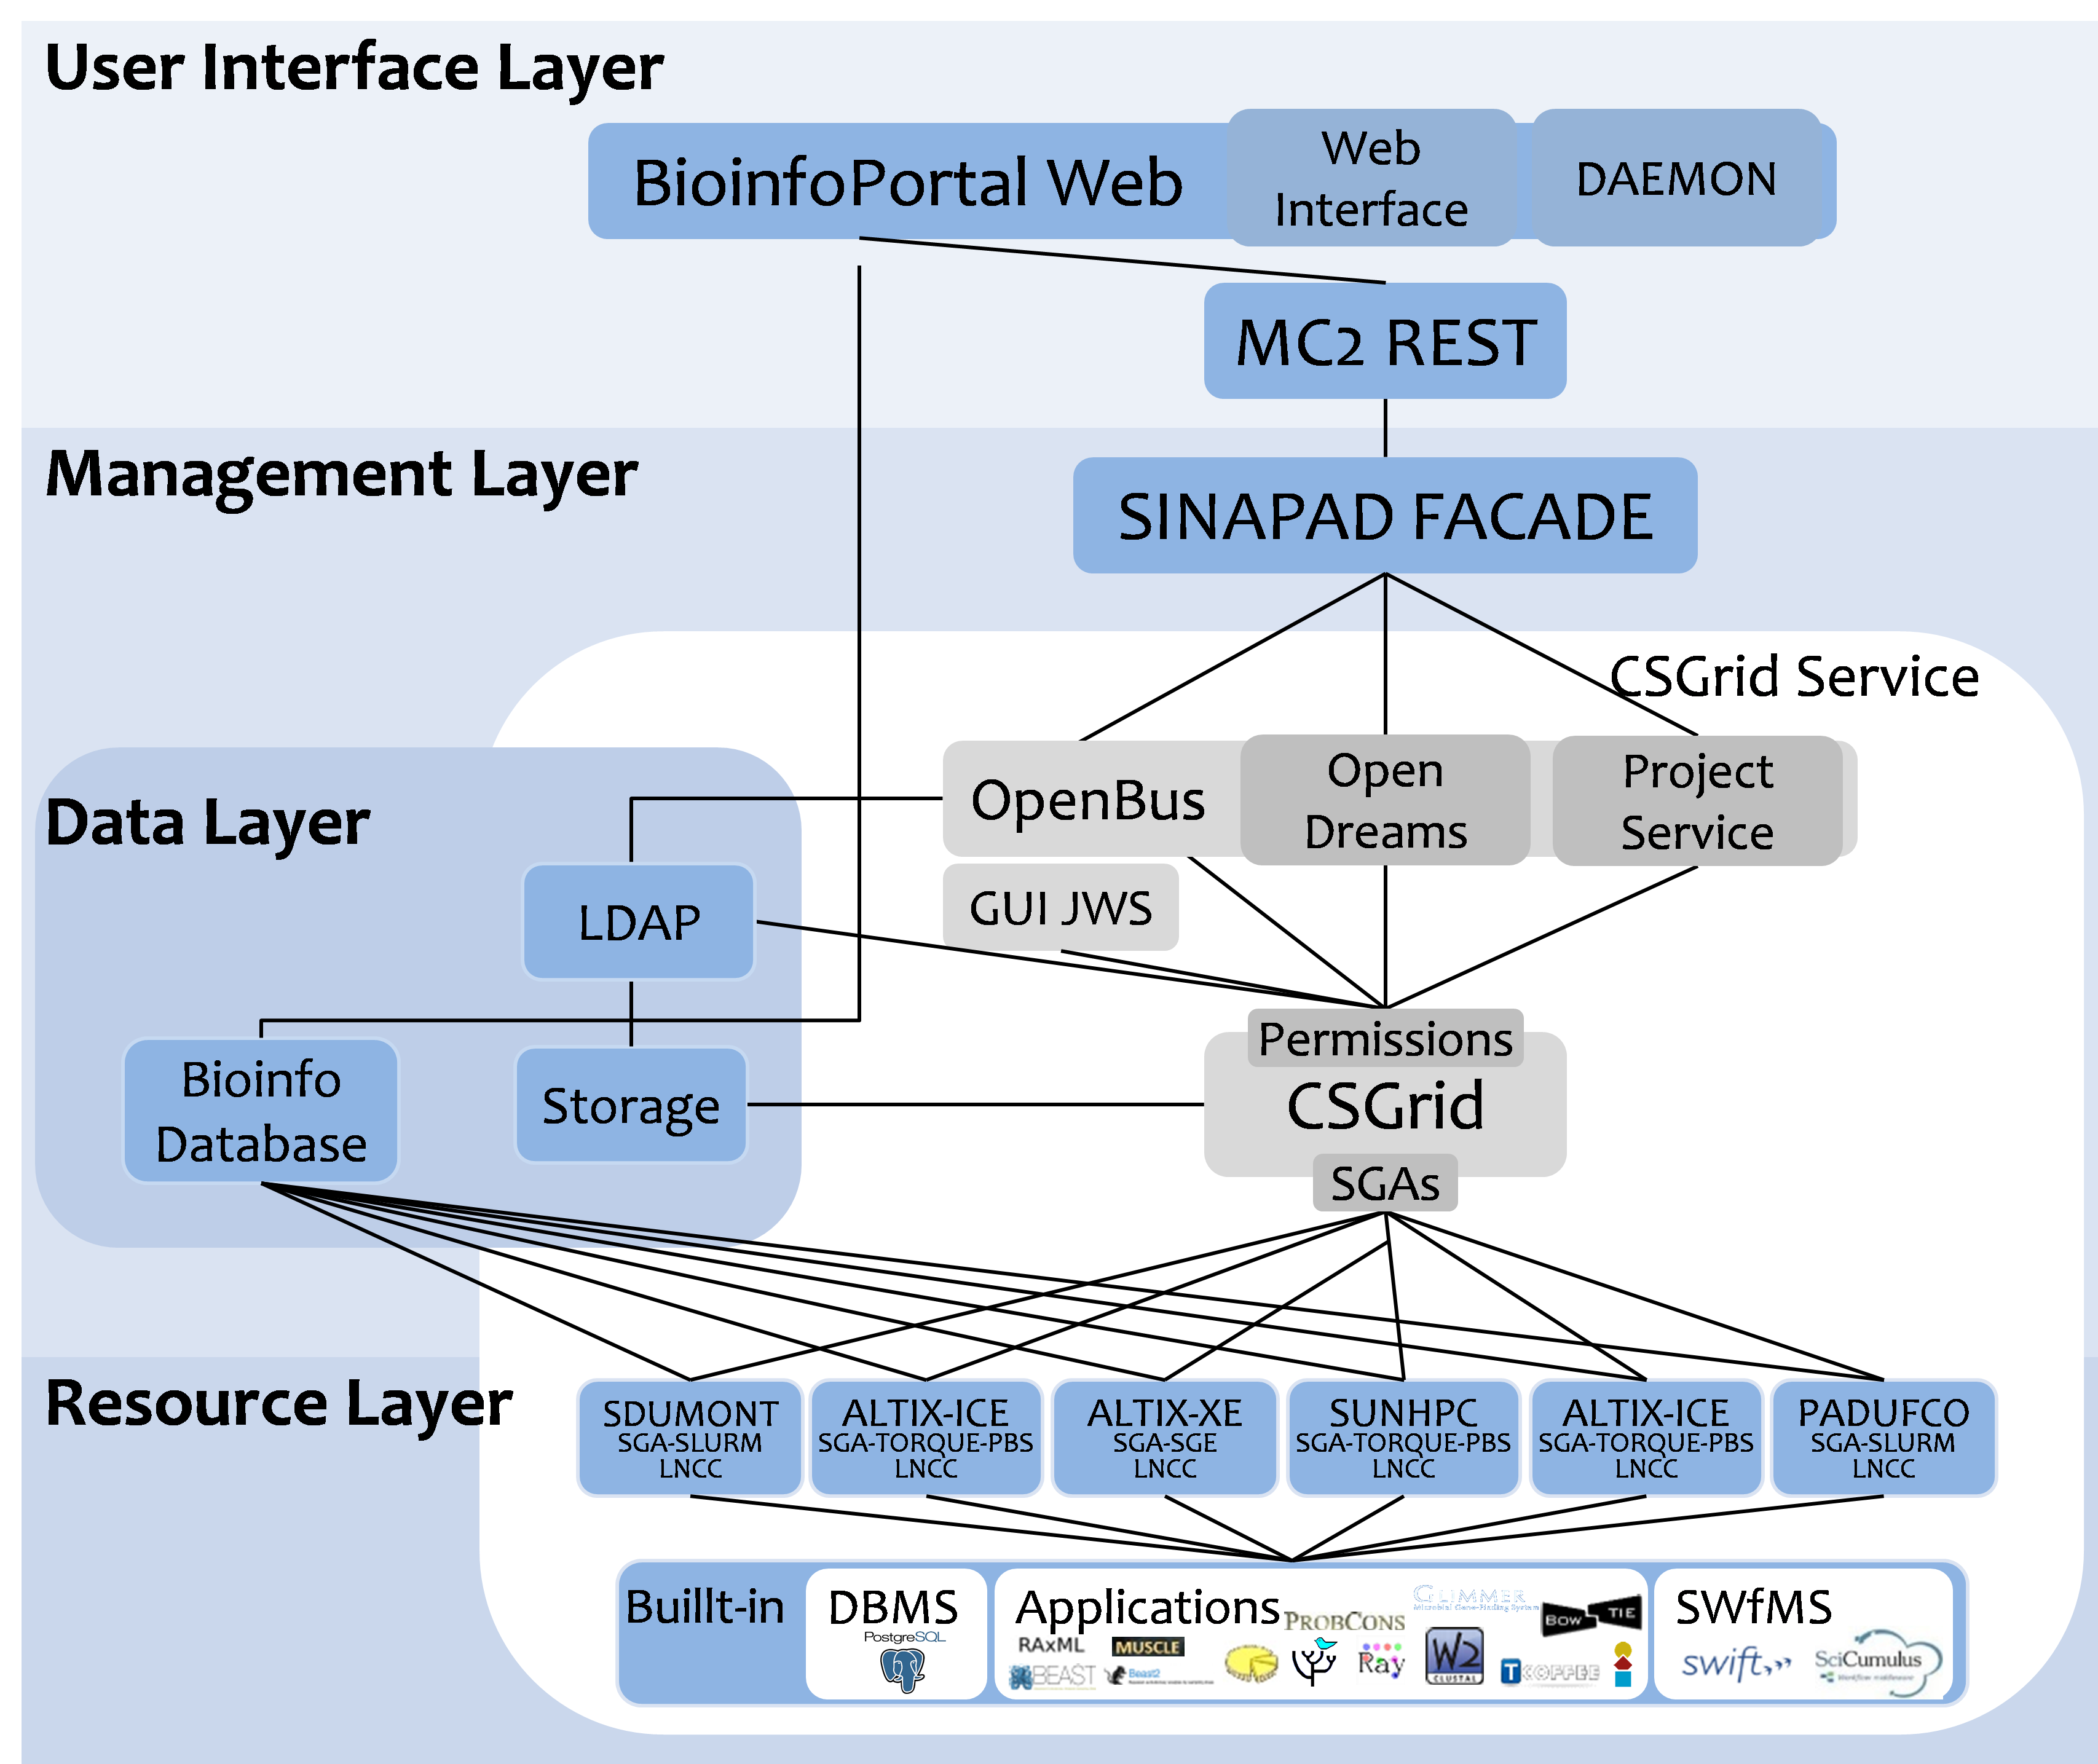
\includegraphics[width=0.75\textwidth]{imgs/bioinfoportal.png}
\vspace{-10px}
\caption{The \system architecture.}
\label{fig:bioinfoportal}
\end{figure*}

\subsection{The User Interface Layer (front-end)}

SINAPAD host several services and portals, as our science gateway \system and presents two main sub-layers: services and applications. \textbf{Services Sub-Layer} is composed of the MC2 services \cite{doi:10.1002/cpe.3258}, as the MC2 REST which dynamically interacts with other services provided by SINAPAD. \textbf{Applications Sub-Layer} is composed of web clients, such as our \system and presents two components: the Web interface and DAEMON. The Web Interface component is used as front-end by users and has an authentication strategy that categorizes the type of access (public or private) assigned to users, which need to be previously registered at SINAPAD through an electronic form. The public access (for guest users) is provided with no authentication, but the service administrator can restrict options for using the computing resources. The private access (for private users) is provided with authentication as the service administrator provides more flexibility or no restriction. The DAEMON component is a robust fault tolerance mechanism for dispatching and scheduling jobs/workflows. DAEMON is connected to the Data Layer at Bioinfo Database for providing an entry for accessing the provenance data information (records of executions or specific domain-data provenance of bioinformatics applications).
The actual version of \system has public access that allows users to choose software, parameters, and input data for submitting their jobs/workflows with no previous authentication.

\vspace{-5px}
\subsection{The Management Layer}

This layer is composed of three sub-layers: Facade, Bus Services, and CSGrid. \textbf{Facade Sub-Layer} enables the configuration for connecting the services (\system, SINAPAD’s services, HPC resources); searches the information needed for applications, clients, and users’ authentication; manages files; and submits/monitors jobs and resources. \textbf{Bus Services Sub-Layer} is implemented as a service-oriented software, called OpenBus, that allows for searching and publishing services by the client applications and for controlling the authentication/authorization of clients and services using internal governance management systems, digital certifications, and LDAP. \textbf{CSGrid Sub-Layer} is a client application of the OpenBus services (OpenDreams, ProjectService) that executes and manages data in the grid environment. CSGrid manages computational resources, clients, users, submissions, data, applications, and user databases (locally or LDAP) of \system at SINAPAD. CSGrid uses the Java-based graphical user interface (GUI) that allows SINAPAD to manage and implement internal applications. CSGrid presents three main conceptual definitions, more information please at XXX: Module, Concept, and Requisition. 

The \textbf{SGA Module} of CSGrid remotely manages the access of computational resources (Resource Layer). SGA is responsible for managing, submitting, scheduling, deleting, associating, and executing computational resources and jobs. SGA uses a pattern nomenclature, which is specific for each application executed in each cluster (sga-<sinapadName>-<schedulerType>-<resourceName>-<queueName>). SGA defines the best combination of settings (name, scheduler type, queue submission, parameters) to maintain the effective connectivity between SINAPAD’s computational resources.

The \textbf{Sandbox Concept} is a mechanism associated with the execution of the computational resources. It provides the availability, reliability, and security of the data using two stages: the stage-in allows users to submit the input data sets and the stage-out returns the results of the executions to the users of a Project at CSGrid. Figure~\ref{fig:raxmlalgorithm} presents the \textbf{Algorithm Concept} that is the structure at CSGrid where the configuration of the applications are available for users and administrators of \system. Algorithm describes the non-interactive applications (their information, input/output data, parameters) that are dispatched directly by the clients of CSGrid. Algorithm provides the information of applications – name, version, and features of installation/compilation in computational resources and configures the client interface. For instance, as the application Align-m was installed in the clusters sun.hpc, altix-xe, ice, sdumont; then the Algorithm Align-m can be created at CSGrid and consequently. This way, all interfaces of SINAPAD as our \system (or others services) are able to access the Algorithm Align-m, to call it, and execute the application Align-m in the clusters sun.hpc, altix-xe, ice, or sdumont.

The \textbf{Requisitions} of SINAPAD allow selecting the computational resources that are available and free at the moment. There are two modes of Requisitions: by users who need to choose the parameters, configurations, and clusters or by schedulers which automatically decide which resource is eligible for submissions. The metric used for schedulers is the number of free Central Processing Units (CPUs) in each cluster. Other metrics as the amount of free memory, disk space, network latency, or job submissions can be included by implementing new plugins. The configuration of the actual version of \system uses public access (no user authentication) with automatic submissions using the mode of the automatic mode by schedulers, but it can be also re-configured.

\vspace{-5px}
\subsection{The Data Layer}

This layer presents four sub-layers the LDAP, Storage, Bioinfo Database, and Scientific Workflow Management Systems (SWfMS) Databases. The \textbf{LDAP Sub-Layer} manages the authentication of users for the portals of SINAPAD. The \textbf{Storage Sub-Layer} stores the information of the user data, application credentials, algorithm configurations, user/application permissions, and execution history proceeding of the application portals and CSGrid. The \textbf{Bioinfo Database Sub-Layer} stores the information (job monitoring, tasks executions, provenance data) proceeding of the applications executed in SINAPAD resources. The The \textbf{SWfMS Database Sub-Layer} includes the provenance databases of the SWfMS SciCumulus \cite{5557969} and Swift \cite{article}. 

The management of the provenance data \cite{e2df054d304d4601be3c733a9d73ff5d} records the history of executions and supports the analysis of scientific experiments. The SciCumulus database follows the data model PROV-Df and W3C PROV and uses the PostgreSQL Relational Database Management System (RDBMS) to manage at runtime the provenance data information consisting of the performance of executions, structure of workflows, and domain-data. Swift is a script programming language for scientific workflows. It uses the server-less SQLite relational database for storing the provenance data. 
The decision-making or fault-tolerance predictions are possible by extracting the provenance information from the databases of Bioinfo and SWfMS and by coupling data mining and machine learning techniques. For instance, provenance information about which tasks are running in which clusters or if the capacity of processing time and memory is enough could be used to predict/prevent errors of executions. Those errors could affect the functionality of services and portals of SINAPAD (including \system) and must be detected. 

\vspace{-5px}
\subsection{The Resource Layer}

The computational resources of SINAPAD are formed by clusters, grids, and public/private clouds. A heterogeneous HPC cluster environment can contain processors and devices with different bandwidth and computational capabilities. Due to that reason, the installation or compilation of the applications and dependencies is made manually by developers/clients, following some requirements: (i) using parameters that optimize the compilation and installation of applications, libraries, and dependencies; (ii) using, as possible, mechanisms and technologies to distribute and parallelize tasks, \textit{i.e.} graphics processor unit (GPU), message passing interface (MPI), or threads; (iii) using mechanisms for optimizing the submissions of schedulers Torque/PBS, SGE, SLURM, Load Leveler; (iv) optimizing the use/configuration of parameters for SWfMS; and (v) coupling to Data Layer, resources as DBMS to register the provenance.

The Resource Layer presents two sub-layers. The \textbf{Applications Sub-Layer} formed by 35 software installed, compiled, and deploted in each cluster of SINAPAD. The \textbf{SWfMS Sub-Layer} formed by the SWfMS SciCumulus \cite{5557969} and Swift \cite{WILDE2011633}, which greatly reducing the complexity of managing experiments by providing features for scalable execution, scalable data management, fault-tolerance, and provenance data tracking \cite{mattoso2010}. The integration of the SWfMS to middleware CSGrid, and the computational resources of SINAPAD require steps, detailed as follows. For SciCumulus, we implemented: (i) a network proxy that allows accessing to the SciCumulus provenance database; (ii) modification of the scripts of configuration (XML) and execution of applications (bash scripts) of SciCumulus, (iii) new bash scripts for mining labels (“tags” in the XML scripts of SciCumulus); and (iv) a connection between the databases of SWfMS and Bioinfo sub-layers. For Swift, we implemented bash scripts to (i) configure Swift at the HPC resources of SINAPAD; (ii) connect the database SQLite to CSGrid and SINAPAD; and (iii) configure the environment to manage execution jobs from a submission node to the clusters.

\vspace{-10px}


\section{\system experimental evaluation}\label{sec:experiments}
\vspace{-2px}
Aiming at evaluating \system, we executed software \raxml and workflows \sci, and \swift with distinct features and took a set of performance measures regarding:
\textit{(i)}~\underline{Performance on \system}, which expresses the overall execution of applications on HPC infrastructures, and 
\textit{(ii)}~\underline{Machine learning data analytics}, which illustrates \system capabilities based on the provenance data of application execution and data feature. Provenance gathered from the executions were stored into a \texttt{Bioinfo} database. As the final part of experimental evaluations, we present \system data analytics reports over an interactive \textit{web} front-end as well as discuss performance and scalability of the applications \raxml, \sci, and \swift in HPC clusters and how information of provenance data can support efficiently the allocation of HPC resources at \system. We presented machine learning technique analyses for predicting the best features (size of input data, software parameters, efficiency) to allocate computational resources on \system.

\subsection{Bioinformatics Software and Workflow Setup}

We experimented on three bioinformatics applications with distinct features regarding activities and performance requirements. \raxml~\cite{sciphy} is an open source software based on Maximum Likelihood (ML) algorithms for statistical calculations to construct trees used for inferring evolutionary life and phylogenetic relationships between genomes.
\sci~\cite{sciphy} is a workflow for phylogeny managed with the SWfMS SciCumulus, which aims at producing phylogenetic trees from input DNA, RNA, and amino acid sequences. 
\swift~\cite{montage} is workflow for parallel genome comparison managed with the SWfMS Swift parallel scripting system, which aims to identify blocks of large rearrangements, starting with the simple collection of ungapped local alignments. In Bioinformatics, comparative and evolutionary analyses of genomes is a traditional problem with high memory and CPU time requisites. Those requisites can be reduced using HPC techniques in its development.
The description of the software \raxml and the conceptual view of the workflows \sci and \swift can be summarized as follows. 

\vspace{5px}
\noindent
\underline{\textbf{\raxml}} is a software of phylogeny based on ML algorithm. It presents four options of execution using multi-core shared memory systems: one sequential and three parallel using MPI, PThreads, or Hybrid (MPI + PThreads) instructions. The sequential version is used to process small to medium datasets and the parallel versions for phylogenomics. The compilation of the code of RAxML was adapted to the capabilities of the CPU infrastructures. Depending on the processor features, RAxML supports three instructions which accelerate the likelihood and parsimony computations: Streaming SIMD Extensions 3 (SSE3), Advanced Vector Extensions (AVX), and AVX2 vector. The parallel efficiency of the PThreads version depends on the alignment length. However PThreads works well for long alignments, the performance is extremely hardware-dependent. The efficiency depends on the number of states of the data; the more states the data have (4 for DNA, 20 amino acid), the fewer site patterns are needed for an efficient parallel execution per thread/core. The parallel efficiency also depends on the rate of heterogeneity of the model; the GAMMA model entails more computations than the CAT model, which needs approximately 1/4 of the computations than the GAMMA model requires. 

Figure~\ref{fig:raxmlalgorithm}(A) presents the web interface of \raxml at \system and Figure~\ref{fig:raxmlalgorithm}(B) presents the layout of the \raxml Algorithm at CSGrid. The web interface of \raxml is automatically generated using the script of configuration \textit{config.xml} presented in Figure~\ref{fig:configxmlcoderaxml} and the scripts of execution \textit{execute.sh} presented in Figure~\ref{fig:executeshcoderaxml} and \textit{prescript.sh} presented in Figure~\ref{fig:prescriptshcoderaxml}. The arguments required to execute \raxml through \system are defined by users, which must upload the input file (alignment in PHYLIP format) and fill options as input file type (nucleotide or amino acid), bootstrap value (default 100), substitution model (GTRGAMMA for nucleotide or PROTGAMMAWAG for amino acid), e-mail, and the output directory. Three experiments with \raxml were performed in Altix and SDumont. The maximum number of cores per node for Altix is 12 and for SDumont is 24. \raxml was compiled with SSE3 in Altix and with AVX in SDumont.

\begin{figure}[!t]
\begin{center}
	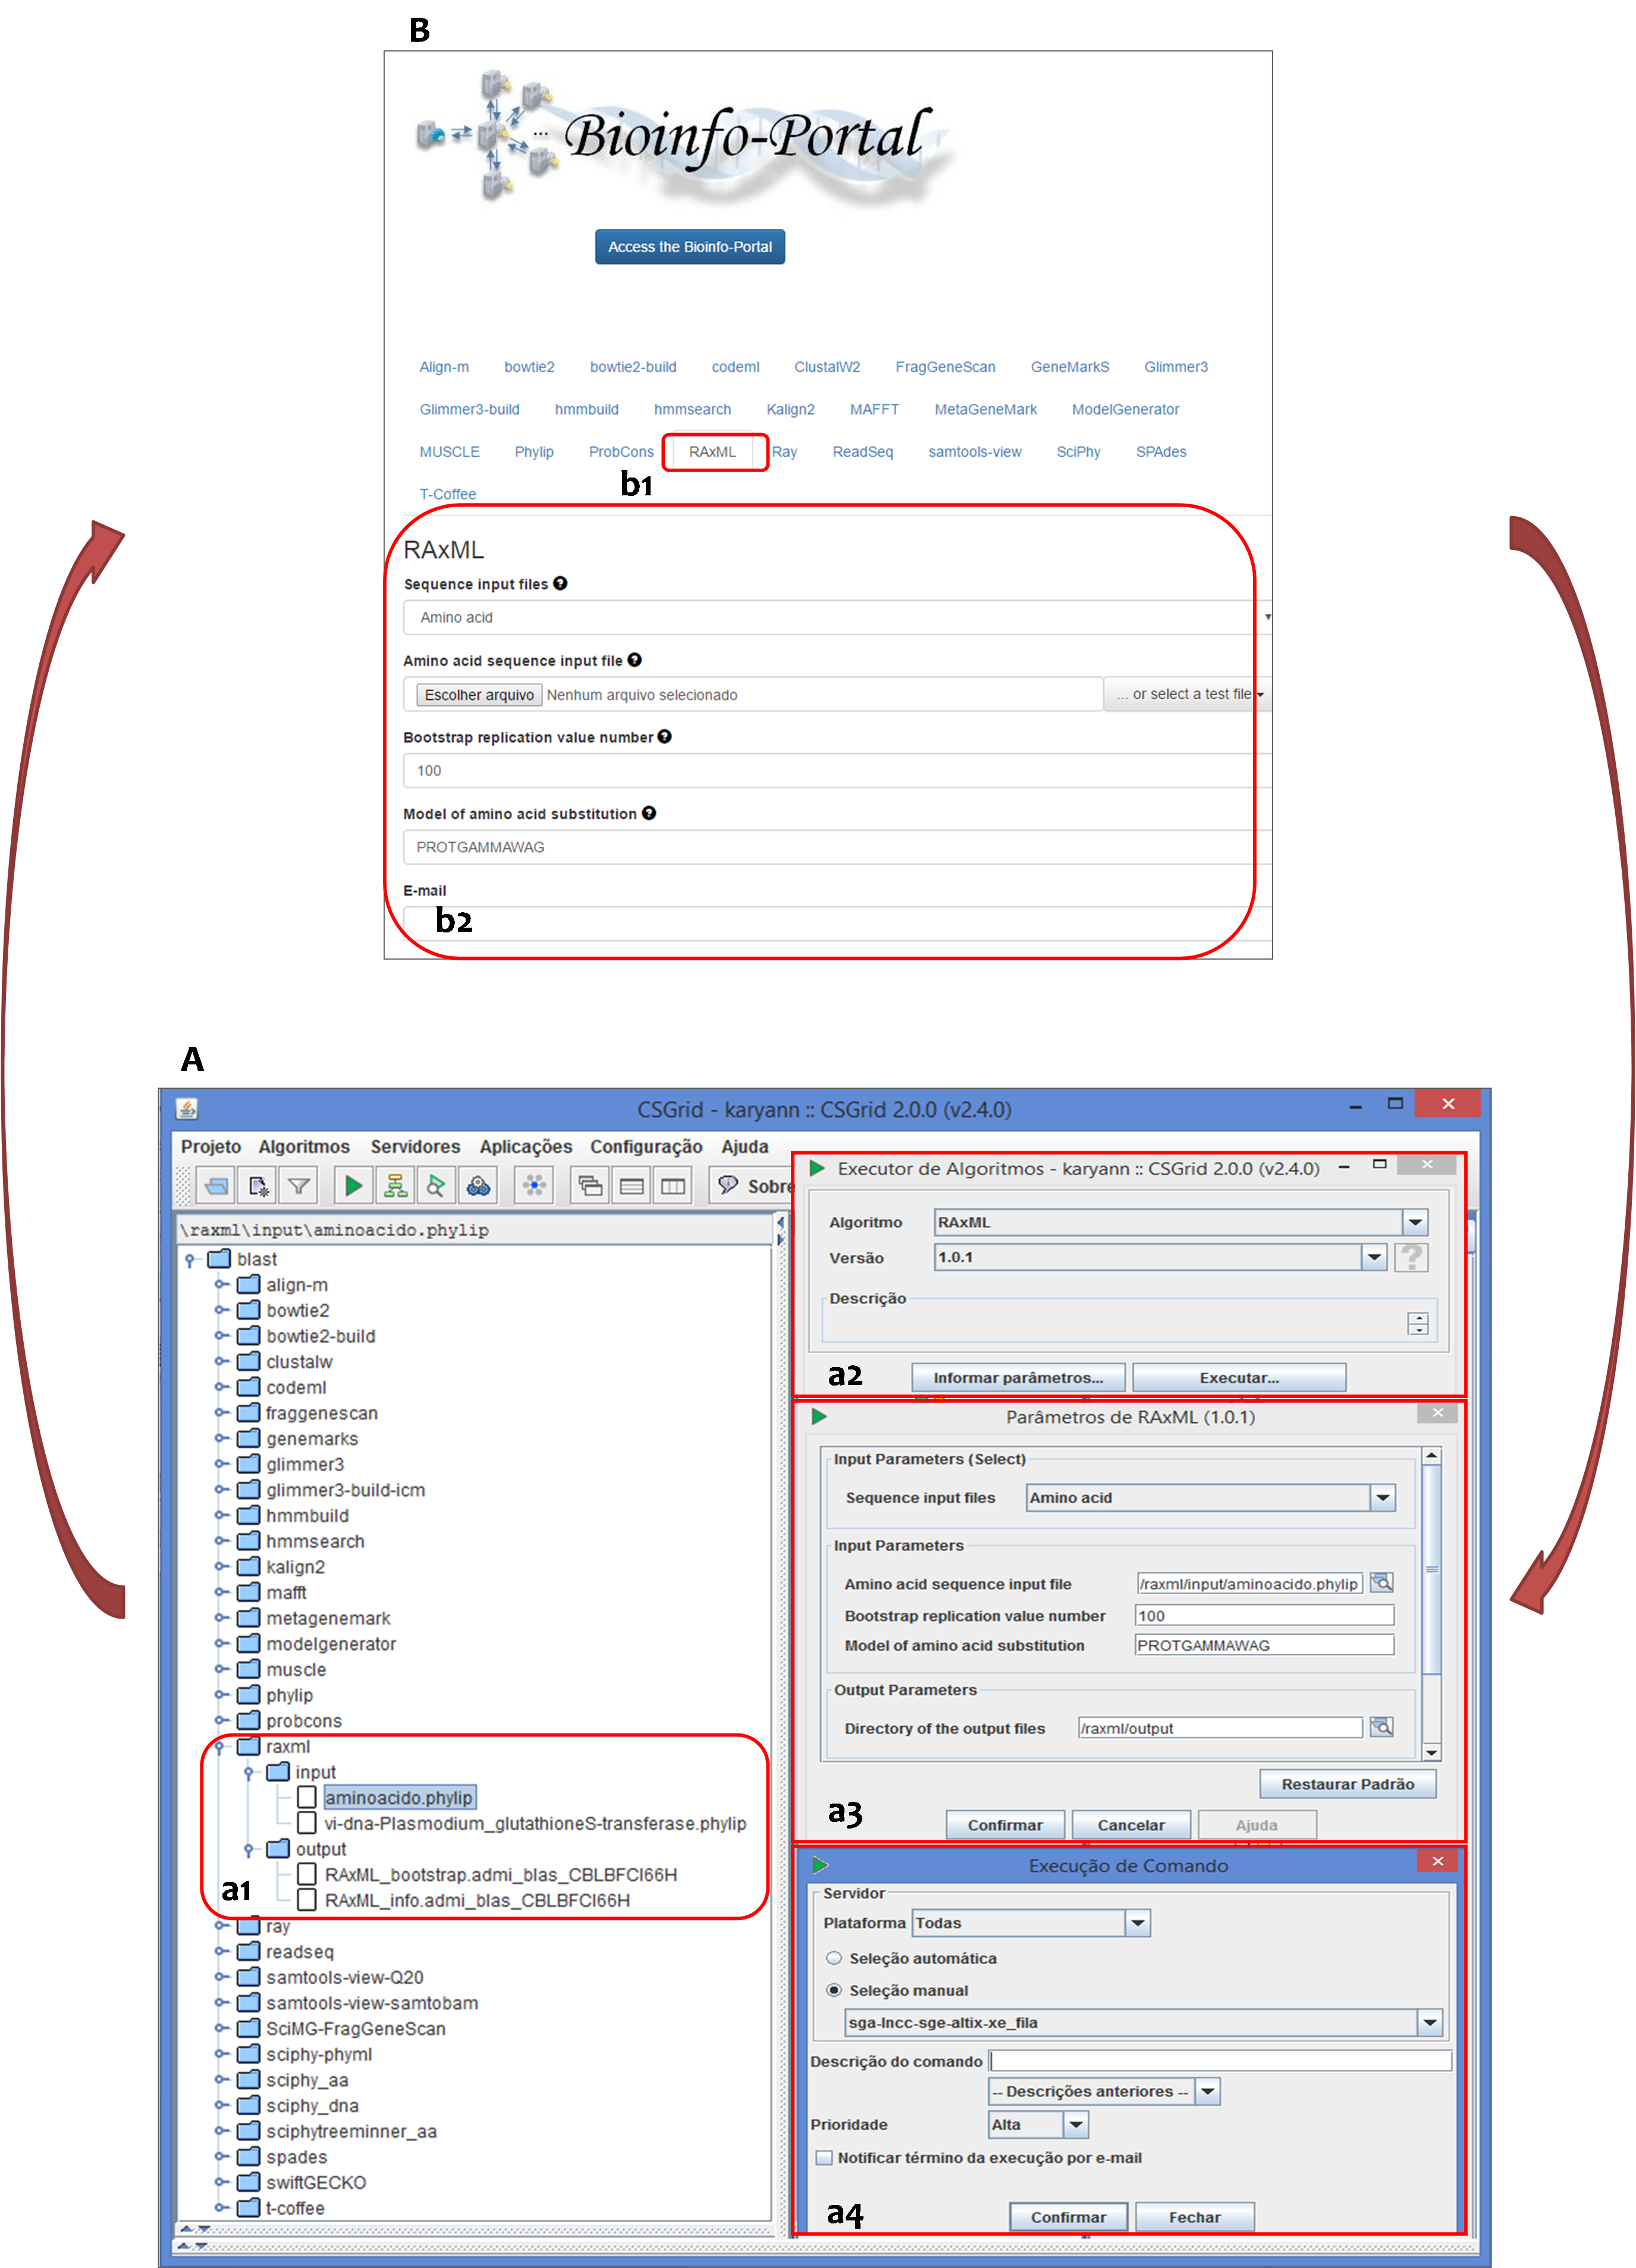
\includegraphics[height=10cm]{imgs/raxmlalgorithm.png}
	\vspace{-7px}
\caption{The Algorithm of the software ~\raxml at the \system front-end.} \label{fig:raxmlalgorithm}
\end{center}
\end{figure}

\vspace{5px}
\noindent
\underline{\textbf{\sci}} is a bioinformatics workflow that aims at constructing ML phylogenetics trees and takes as input data sequences of DNA, RNA, or amino acid. \sci is managed with the SWfMS SciCumulus and its execution is computationally intensive. Figure~\ref{fig:sciphyworkflow} illustrates the \sci workflow, which essentially consists of three sequential activities followed by two concurrent activities, all implemented by black-box and external programs.
The pipeline can be summarized by the following activities:
\textit{(i)}~multiple sequence alignment, implemented by the MAFFT program, 
\textit{(ii)}~alignment format conversion, conducted through the ReadSeq program, 
\textit{(iii)}~best evolutionary model election, carried out by the ModelGenerator program, 
\textit{(iv)}~phylogenetic tree construction, implemented by the RAxML program. 
Since each one of these activities performs a parameter sweep individually, they generate several independent tasks.

\begin{figure}[!t]
\begin{center}
	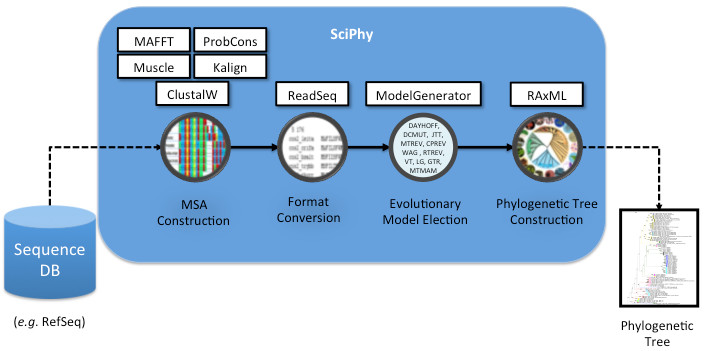
\includegraphics[height=7.7cm]{imgs/sciphyworkflow.png}
	\vspace{-7px}
\caption{The conceptual view of the workflow ~\sci with activities.} \label{fig:sciphyworkflow}
\end{center}
\end{figure}

SciCumulus’ provenance database stores domain data related to the workflow \sci. It is connected to the \system database at CSGrid, which provides the access to the information of other \system applications as well as to other services/portals at CSGrid/SINAPAD. As SciCumulus queries the provenance database at runtime, the Web interface of \system automatically will report messages of the \sci execution status \textit{e.g.} which activity is finished or if any error is presented. 
Figure~\ref{fig:sciphyalgorithm} shows the \sci Web interface at Bioinfo-Portal. This layout is automatically generated based on the configuration scripts config.xml (Additional file 4), execute.sh (Additional file 7), and prescript.sh (Additional file 8). The input arguments required by \sci at \system are one input file (\textit{e.g.} alignment in FASTA format), one selection option for input file type (\textit{e.g.} amino acid), an e-mail address, and one directory for output files. 

\begin{figure}[!t]
\begin{center}
	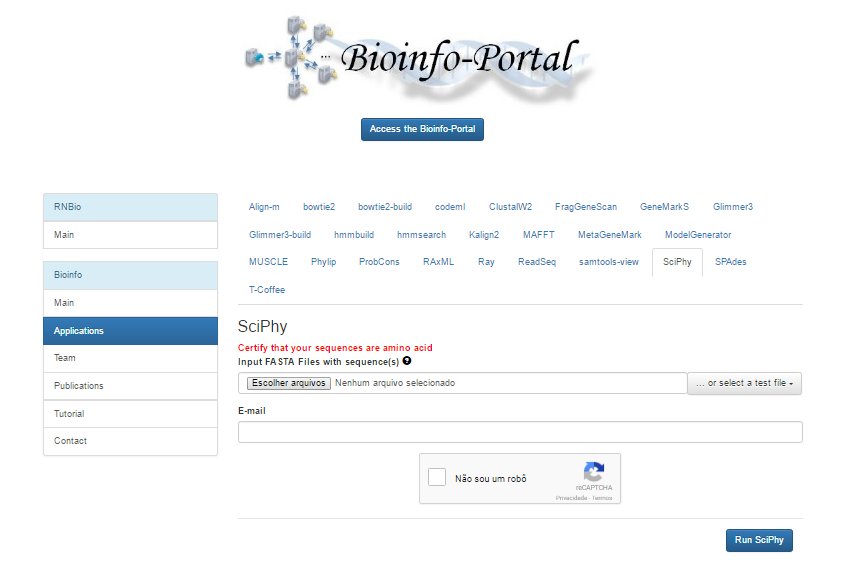
\includegraphics[height=8.7cm]{imgs/sciphyalgorithm.png}
	\vspace{-7px}
\caption{The Algorithm of the software ~\sci at the \system front-end.} \label{fig:sciphyalgorithm}
\end{center}
\end{figure}

\vspace{5px}
\noindent
\underline{\textbf{\swift}} is the workflow that maps the application GECKO {REF} using the SWfMS Swift which provides task-level parallelization and provenance data tracking. GECKO was designed to identify collections of high-scoring segment pairs (HSPs) by genome comparisons.Figure \ref{fig:swiftgeckoworkflow} describes the three modules of the workflow \swift that is composed at total for ten activities:
\textit{(i)}~Dictionary Calculation, which created dictionaries for the sequence input data; it is composed of activities 1-4,
\textit{(ii)}~high-scoring segment pairs (HSP) Detection, which detects hits used to identify the HSP locations; it is composed activities 5-9, in green boxes, and
\textit{(iii)}~Post-processing, which performs statistical calculations and functional annotations; it is composed by the activity 10, in the orange box.
\vspace{5px}

\begin{figure}[!t]
\begin{center}
	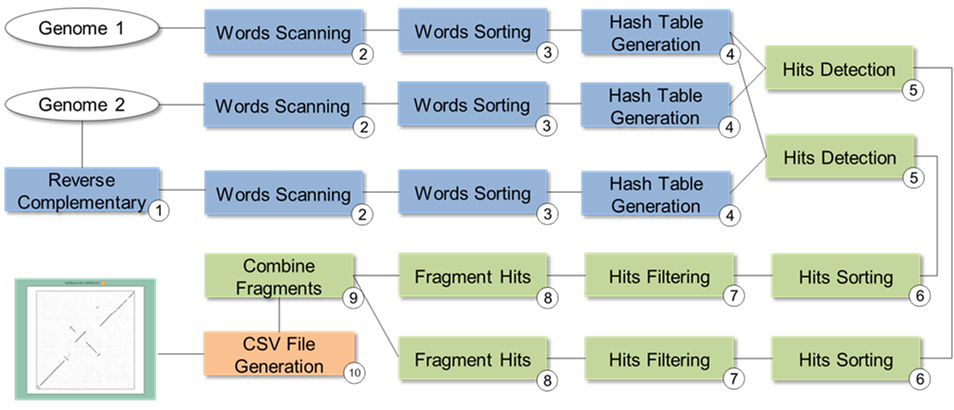
\includegraphics[height=6.7cm]{imgs/swiftgeckoworkflow.png}
	\vspace{-7px}
\caption{The conceptual view of the workflow ~\swift with activities.} \label{fig:swiftgeckoworkflow}
\end{center}
\end{figure}

The provenance database of \swift stores the provenance data information as the TET and the scientific domain data information. By querying the provenance database of Swift, specialists can infer about the evolutionary and taxonomic relationship of genomes based on the number of fragments, also crossing with computational information of CPU consumed. The input arguments required by \swift at \system, are one input file (genomes in FASTA format), one selection option for GECKO parameters (length, similarity, word length, FixedL), and an e-mail.
Figure~\ref{fig:swiftgeckoworkflow} shows the \swift Web interface at \system and the input arguments required are one input file \textit{i.e.} the genomes, the parameters of GECKO and the user's e-mail for returning results.

\begin{figure}[!t]
\begin{center}
	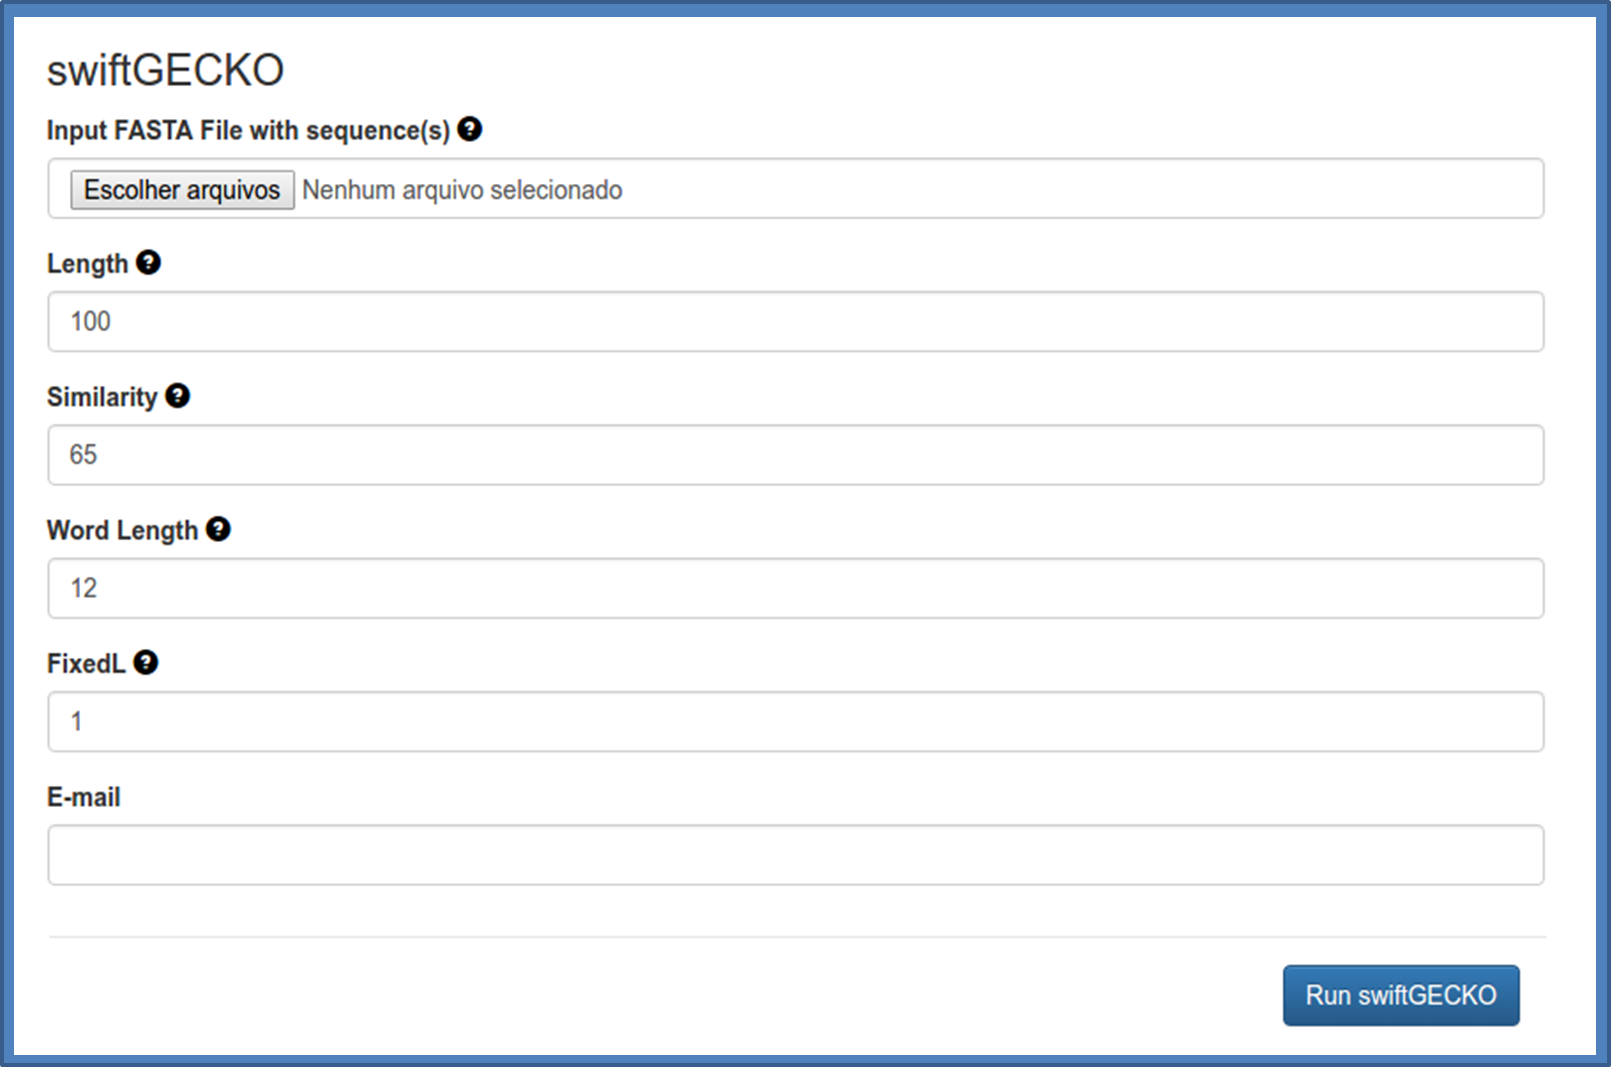
\includegraphics[height=7.7cm]{imgs/swiftgeckoalgorithm.png}
	\vspace{-7px}
\caption{The Algorithm of the software ~\swift at the \system front-end.} \label{fig:swiftgeckoalgorithm}
\end{center}
\end{figure}

\subsection{Experimental Data and Setup} \label{expsetup}
The experiments of ~\raxml, ~\sci, and ~\swift were executed in the cluster Altix ICE\footnote{\url{http://www.lncc.br/ice/}} and supercomputer SDumont\footnote{\url{http://sdumont.lncc.br/}}. Altix consists of 25 diskless machines (execution nodes), each node is given by an SGI ICE 8400 server with 2 Intel Xeon X5650 2.67GHz Hexa Core processors (totaling 12 cores) and 48 GB DDR3 DIMMs of memory. The cluster has one login node with a gross storage capacity of 5TB. SDumont consists of 16 TB RAM, storage totaling 1,7 PetaBytes (Seagate 1.5 Buster), 10.692 cores, 1.1 PetaFlops, Intel Xeon E5-2695v2, 30 MB cache, 12 cores – 3.2 GHz.

\underline{\textbf{\raxml}} experiment data is formed by amino acid superalignments in format PHYLIP. Table~\ref{tab:superalignments} presents the features of the superalignments used as input data for the execution of \raxml. The eight superalignment files were categorized as Large (D1, D2), Medium (D3, D4, D7, D8), and Small (D5, D6). This classification was based on the features of the alignment sequences as the Number of Taxa, Number of Amino Acid, and Size in KB. For example, the input file D5 has a size of 79 KB and it is formed of 31 concatenated universal orthologous (UO) genes from 12 protozoan genomes. \underline{\textbf{\sci}} experiment data are input file of amino acid sequences of 200 multi-fasta alignments in FASTA format. The biological sequences used for constructing phylogenetic trees are orthologous genes of 12 protozoan genomes. \underline{\textbf{\swift}} experiment data are input file of amino acid sequences of eight mammalian genomes in FASTA format. 

\begin{table}[!t]
\centering
\caption{Comparison of alternatives for provenance support in Spark.}
\label{tab:superalignments}
\resizebox{\textwidth}{!}{\begin{tabular}{|l|p{2.2cm}|p{2.2cm}|p{2.2cm}|p{2.2cm}|p{2.2cm}|p{2.2cm}|}
\hline
\multirow{2}{*}{} & \multicolumn{4}{c|}{\textbf{Features}} \\ \cline{2-5} 
                      & \textbf{Category} & \textbf{Number of Taxa}  & \textbf{Number of Amino Acid}  & \textbf{Size in KB}     \\ \hline\hline
                      
\textbf{Superalignment D1}    
& Large   & 74   &  21,260   &  2,091   \\ \hline
\textbf{Superalignment D2}      
& Large   & 74   &  12,807   &  1,260   \\ \hline
\textbf{Superalignment D3}      
& Medium   & 26   &  22,906   &  792   \\ \hline
\textbf{Superalignment D4}       
& Medium   & 26   &  16,068   &  553   \\ \hline
\textbf{Superalignment D5}     
& Small   & 12   &  4,941   &  79   \\ \hline
\textbf{Superalignment D6}     
& Small   & 12   &  4,481   &  72   \\ \hline
\textbf{Superalignment D7}     
& Medium   & 36   &  3,490   &  168   \\ \hline
\textbf{Superalignment D8}     
& Medium   & 36   &  3,270   &  157   \\ \hline
\end{tabular}}
\end{table}

\subsection{\system settings: the architecture of the science gateway}

CSGrid provides the central infrastructure for developing the Algorithms and managing executions using the computational resources of SINAPAD. Each Algorithm presents scripts of configuration (“.xml”) and execution (“.sh”), which are modified/implemented following the requirements of the applications or computational resources. The main scripts are \texttt{portal.xml} that configures the main web interface of \system; \texttt{config.xml} that configures the parameters used by each Algorithm; \texttt{execute.sh} that executes the Algorithm based on the parameters of \texttt{config.xml}; and \texttt{prescript.sh} that presents the parameters to configure the environment for the computational resources. Figure~\ref{fig:raxmlmanagement} presents the structure of CSGrid for the Algorithm ~\raxml, the scripts, and the available computational resources.

\begin{figure}[!t]
\begin{center}
	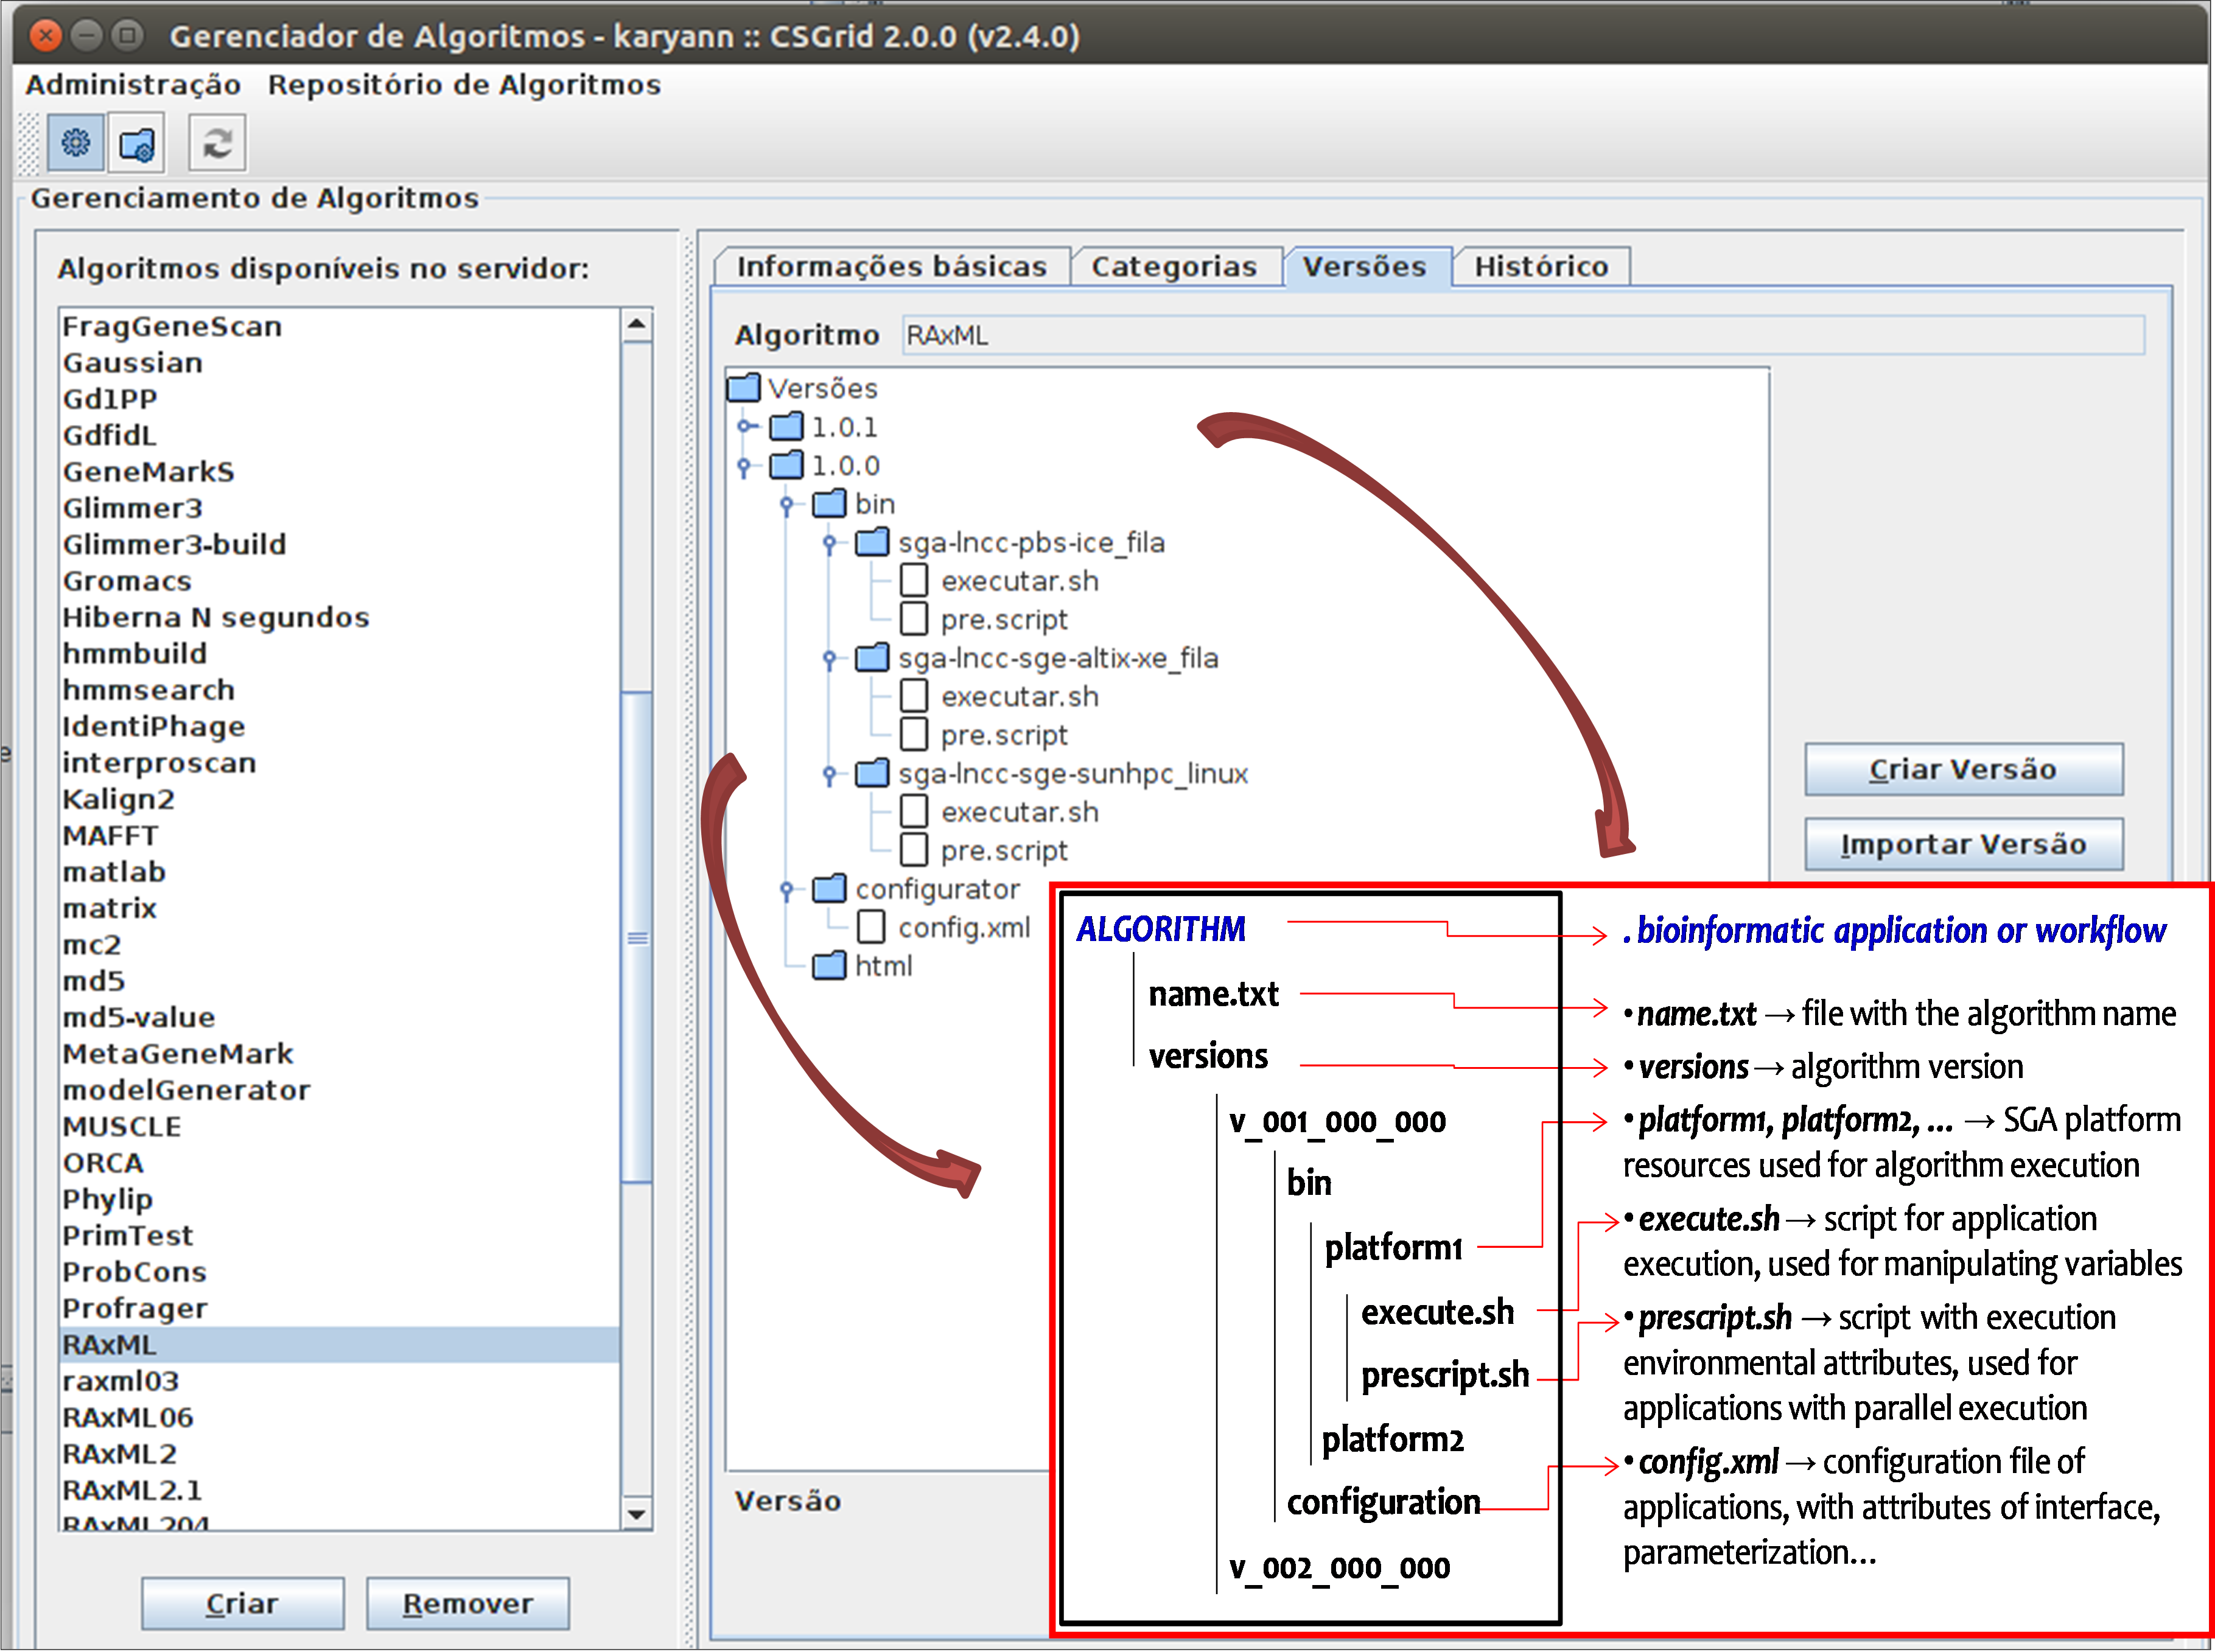
\includegraphics[height=8.7cm]{imgs/raxmlmanagement.png}
	\vspace{-7px}
\caption{The management of the Algorithm ~\raxml at the CSGrid of the \system front-end.} \label{fig:raxmlmanagement}
\end{center}
\end{figure}

\underline{\textbf{portal.xml}} connects the web interface of \system to the Project area of the Algorithms. CSGrid defines which Algorithm will be executed by the gateway. The user must select the Algorithm; then, the web interface is dynamically built in the gateway and provides the fields of input/output and parameters that need to be filled by the user. The \texttt{portal.xml} allows that multiple versions of the same Algorithm be available at the gateway (XML attribute multiple-versions); then users can execute several versions of the applications. The final excerpt of Figure~\ref{fig:portalxmlcode} presents an example of a configuration script invocation, whose parameters are required for the processing of the Algorithms \raxml and \sci in \system. 

 \begin{figure}[!t]
 \begin{lstlisting}[style=myScalastyle]
 // The script portal.xml for RaXML and SciPhy
1    <portal-config multiple-versions="true" resource-choice="true" auto-generate="true">
2            ...
3            <acronym-name>Bioinfo</acronym-name>
4            <full-name>Bioinfo-Portal Gateway</full-name>
5            <csgrid-project-name> Bioinfo </csgrid-project-name>
6            <algorithms-config>
7                    <algorithm>
8                           <name>RAxML</name>
9                           <default-version>1.0.0</default-version>
10                   </algorithm>
11                   <algorithm>
12                           <name>SciPhy</name>
13                           <default-version>1.0.0</default-version>
14                   </algorithm>
15           </algorithms-config>
16           ...
17   </portal-config>

\end{lstlisting}
\vspace{-10px}
\caption{Implementation of the configuration script \texttt{portal.xml} for the invocations of Algorithms \raxml and \sci in \system.}
\label{fig:portalxmlcode}
\end{figure}

\underline{\textbf{config.xml}} describes the input/output arguments required by each Algorithm. It is similar in purpose to the files of the JSON Service Description Language (JSDL) of the middleware UNICORE \cite{ref10.1007/11508380_38} and the Common Tool Description (CTD) of the OpenMS library. Nevertheless, \texttt{config.xml} provides more details about how the arguments of the Algorithm can be rendered in a user interface \textit{e.g.} to the conditional attributes: “for the Algorithm RAxML, the fields A (amino acid type) and B (nucleotide type) are mutually exclusive”. These attributes allow users to hide/disable field(s) at the web interface determined by one specific value of the flag. The \texttt{config.xml} is used by CSGrid for dynamically assembling the web interfaces and by the OpenDreams service for invocating the commands of scripts that reify the Algorithm in the underlying computational resources. The final excerpt of Figure~\ref{fig:configxmlcoderaxml} presents an example of the invocation of a configuration script and whose parameters are required for processing the Algorithm \raxml in \system. Figure~\ref{fig:configxmlcoderaxml} presents the example for invocating the Algorithm \sci in \system. 

 \begin{figure}[!t]
 \begin{lstlisting}[style=myScalastyle]
 // The script config.xml for RaXML
1    <?xml version='1.0' encoding='UTF-8'?>
2    <algorithm command="execute.sh" capture_code_ouput="yes" provide_identifier="yes">
3        <format_command>$NAME_PARAMETER=$VALUE_PARAMETER </format_command>
4        <group label='Input Parameters (Select)'>
5            <enum name="RAXML_INPUTTYPES" label="Input files" clue="Select file(s)"standard="dna">
6                <item_enum id="aa" label="Amino acid" value="aa" clue="Provide amino acid input file"/>
7                <item_enum id="dna" label="Nucleotide" value="dna" clue="Provide nucleotide input file"/>
8            </enum>
9        </group>
10      <group label="Input Parameters">
11          <entire name="numCPU"
              label="CPUs number"
              minimum="1"
              maximum="16"
              clue="Set the number of threads to allocate (min 1 - max 16)"
              standard="16"
              optional="true"/>
12          <file_input name="RAXML_INPUT_AA"
              label='Amino acid sequence input file'
              clue='Select or upload the amino acid sequence input file'/>
13          <file_input name="RAXML_INPUT_DNA"
              label='Nucleotide sequence input file'
              clue='Select or upload the right sequence input file'/>
14          <entire name="RAXML_BOOTSTRAP"
              label="Bootstrap replication value number"
              minimum="1" 
              maximum="2000"
              clue ="Set the number of replication for bootstrap (default 100)"
              standard="100"
              optional="true"/>
15          <text name="RAXML_MODEL_DNA"
              label="Model of nucleotide substitution"
              clue="Model of nucleotide substitution"
              standard="GTRGAMMA"
              optional="true"/>
16          <text name="RAXML_MODEL_AA"
              label="Model of amino acid substitution"
              clue="Model of amino acid substitution"
              standard="PROTGAMMAWAG"
              optional="true"/>
17      </group>
18      <group label='Output Parameters'>
19          <file_output name="RAXML_OUTPUT" 
              label="Directory of the output files" 
              clue="Select the output directory where the result files will be placed" 
              category="directory"/>
20      </group>
21      <display>
22          <parameter name="RAXML_INPUT_DNA"/>
23          <parameter name="RAXML_MODEL_DNA"/>
24          <condition parameter="RAXML_INPUTTYPES" value="dna"/>
25      </display>
26      <display>
27          <parameter name="RAXML_INPUT_AA"/>
28          <parameter name="RAXML_MODEL_AA"/>
29          <condition parameter="RAXML_INPUTTYPES" value="aa"/>
30      </display>
31  </algorithm>
\end{lstlisting}
\vspace{-10px}
\caption{Implementation of the configuration script \texttt{config.xml} for the invocations of Algorithm \raxml in \system.}
\label{fig:configxmlcoderaxml}
\end{figure}

 \begin{figure}[!t]
 \begin{lstlisting}[style=myScalastyle]
 // The script config.xml for SciPhy
1    <?xml version='1.0' encoding='UTF-8'?>
2    <algorithm command="execute.sh" capture_code_ouput="yes" provide_identifier="yes">
3        <format_command>$NAME_PARAMETER=$VALUE_PARAMETER </format_command>
4        <group label="Input Parameters">
5          <file_input name=" SciPhy_INPUT "
              label="Input directory of FASTA file(s)"
              clue="Select or upload the input fasta file(s), not exceed 10 files or 10 Mb in size"
              category="directory"/>
6      </group>
7    <group label='Output Parameters'>
8          <file_output name=" SciPhy_OUTPUT" 
              label="Directory of the output files" 
              clue="Select the output directory where the result files will be placed" 
              category="directory"/>
9      </group>
10  </algorithm>

\end{lstlisting}
\vspace{-10px}
\caption{Implementation of the configuration script \texttt{config.xml} for the invocations of Algorithm \sci in \system.}
\label{fig:configxmlcodesciphy}
\end{figure}

\underline{\textbf{execute.sh}} describes the specific arguments used for the execution of the Algorithms belonging to each one of the bioinformatics applications. The arguments or parameters can be extracted from the command line used to execute the applications. The final excerpt of Figure~\ref{fig:executeshcoderaxml} presents an example for the invocation of a execution script and whose parameters are required for the processing of the Algorithm \raxml in \system. 

 \begin{figure}[!t]
 \begin{lstlisting}[style=myScalastyle]
 // The script execute.sh for RAxML
1    #!/bin/bash
2    . ~/setclasspath.sh
3    . /hpc/modulos/bash/openmpi-1.8.5-gcc47.sh
4    function parseArgs {
5        for arg in $* ; do
6            typeset name=`echo $arg | sed "s/=.*//"`
7            typeset value=`echo $arg | sed "s/.*=//"`
8            export $name=$value
9        done
10  }

 // CSGrid Arguments
11  parseArgs $*
12  echo "Id SGE: "$JOB_ID, $RAXML_INPUTTYPES, $RAXML_INPUT_DNA, $RAXML_INPUT_AA, $RAXML_BOOTSTRAP, $RAXML_MODEL_AA, $RAXML_MODEL_DNA, $RAXML_OUTPUT
13  cmdId=`echo $cmdId | sed 's/\(.*\)\@\(.*\)\.\(.*\)/\1_\2_\3/'`

 // Execute RAxML
14  cd $RAXML_OUTPUT
15  numCPU=$NSLOTS
16  COMMAND="/usr/bin/time -f "%e" -o ${RAXML_OUTPUT}/.time.log 2  $ALGORITHMS_THIRD_DIR/RAxML/versions/v_001_000_000/RAxML/standard-RAxML-master/raxmlHPC-MPI-SSE3"
17  COMMANDmpi="/usr/bin/time -f "%e" -o ${RAXML_OUTPUT}/.time.log mpirun -np $numCPU -hostfile $TMPDIR/hostfile $ALGORITHMS_THIRD_DIR/RAxML/versions/v_001_000_000/RAxML/standard-RAxML-master/raxmlHPC-MPI-SSE3"
18  if [ "$RAXML_INPUTTYPES" == "dna" ]
19  then
 // Best tree
20      EXEC1="$COMMAND -m $RAXML_MODEL_DNA -p 112233 -s $RAXML_INPUT_DNA -n $cmdId.best -c 4 -f d"
21      $EXEC1
 // Bootstrap
22      EXEC2="$COMMAND -m $RAXML_MODEL_DNA -p 112233 -s $RAXML_INPUT_DNA -b 223344 -# $RAXML_BOOTSTRAP -n $cmdId.bootreps -c 4 -f d"
23      $EXEC2
 // Consense
24      EXEC3="$COMMAND -m $RAXML_MODEL_DNA -s $RAXML_INPUT_DNA -f b -t RAxML_bestTree.$cmdId.best -z RAxML_bootstrap.$cmdId.bootreps -n $cmdId.bestML.bootstrap"
$EXEC3
25  fi
26  if [ "$RAXML_INPUTTYPES" == "aa" ]
27  then
 // Best tree
28      EXEC1="$COMMAND -m $RAXML_MODEL_AA -p 112233 -s $RAXML_INPUT_AA -n $cmdId.best -c 4 -f d"
29      $EXEC1
 // Bootstrap
30      EXEC2="$COMMAND -m $RAXML_MODEL_AA -p 112233 -s $RAXML_INPUT_AA -b 223344 -# $RAXML_BOOTSTRAP -n $cmdId.bootreps -c 4 -f d"
31      $EXEC2
 // Consense
32      EXEC3="$COMMAND -m $RAXML_MODEL_AA -s $RAXML_INPUT_AA -f b -t RAxML_bestTree.$cmdId.best -z RAxML_bootstrap.$cmdId.bootreps -n $cmdId.bestML.bootstrap"
33      $EXEC3
34  fi

 // $COMMAND
35  if [ $? != 0 ]
36   then
37      echo "RAxML returned an error."
38      exit 1
39  fi
\end{lstlisting}
\vspace{-10px}
\caption{Implementation of the configuration script \texttt{execute.sh} for the invocations of Algorithm \raxml in \system.}
\label{fig:executeshcoderaxml}
\end{figure}

\underline{\textbf{prescript.sh}} describes the arguments used for the invocation of the script of the configuration of the environment. The final excerpt of Figure~\ref{fig:prescriptshcoderaxml} presents an example for the invocation of the script of execution and whose parameters are required for the processing the Algorithm \raxml in \system. 

 \begin{figure}[!t]
 \begin{lstlisting}[style=myScalastyle]
 // The script prescript.sh for RAxML
1    #$ -N JOB_RAXML
2    #$ -cwd
3    #$ -V
4    #$ -pe mpi 16
5    #$ -l h_rt=216000
\end{lstlisting}
\vspace{-10px}
\caption{Implementation of the configuration script \texttt{prescript.sh} for the invocations of Algorithm \raxml in \system.}
\label{fig:prescriptshcoderaxml}
\end{figure}


\subsection{Performance on \system}
As the first \system evaluation, we measured the performance and scalability of executions of the applications \raxml, \sci, and \swift. Every experiment of applications was evaluated separately in order to highlight the impact of each feature individually. We executed all experiments of \system in SDumont clusters. Additionally, all executions provenance data were used as input information for executing machine learning analyses in order to determine the general features of application executions according to input size, software parameters, and efficiency that better offer requirements for optimizing the allocation of machines capacity for experiments.

\vspace{5px}
\noindent
\underline{\textbf{\raxml} Performance Analyses}

\textit{1) The total execution time of the versions of \raxml}. The \raxml HPC Serial was executed in one single core, \raxml PThreads in 12 cores, \raxml MPI in 120 cores, and \raxml Hybrid in 120 cores. The input file used in this experiment was the amino acid superalignment D5 in format PHYLIP, with a size of 79 KB and formed of 31 concatenated universal orthologous (UO) genes from 12 protozoan genomes. The parameters used for setting the \raxml versions are JTT as the evolutionary model, GAMMA as the rate of model heterogeneity, and 100 as the bootstrap value of replications. Figure~\ref{fig:raxmlTETD5} presents the Total Execution Time (TET) in minutes obtained after the execution of the versions of \raxml. The TET decreases using the parallel versions PThreads, MPI, and Hybrid of \raxml in comparison to the version \raxml HPC Serial and using the clusters of SDumont compared to Altix. For Altix, the \raxml MPI was the version that presented the best performance, with the TET reduced from 285,57 minutes (one single core) to 4.59 minutes (using 120 cores). For SDumont, the \raxml Hybrid was the version that presented the best performance, with the TET reduced from 161,29 minutes (using one single core) to 1.88 minutes (using 120 cores). 

\begin{figure}[!htb]
\centering
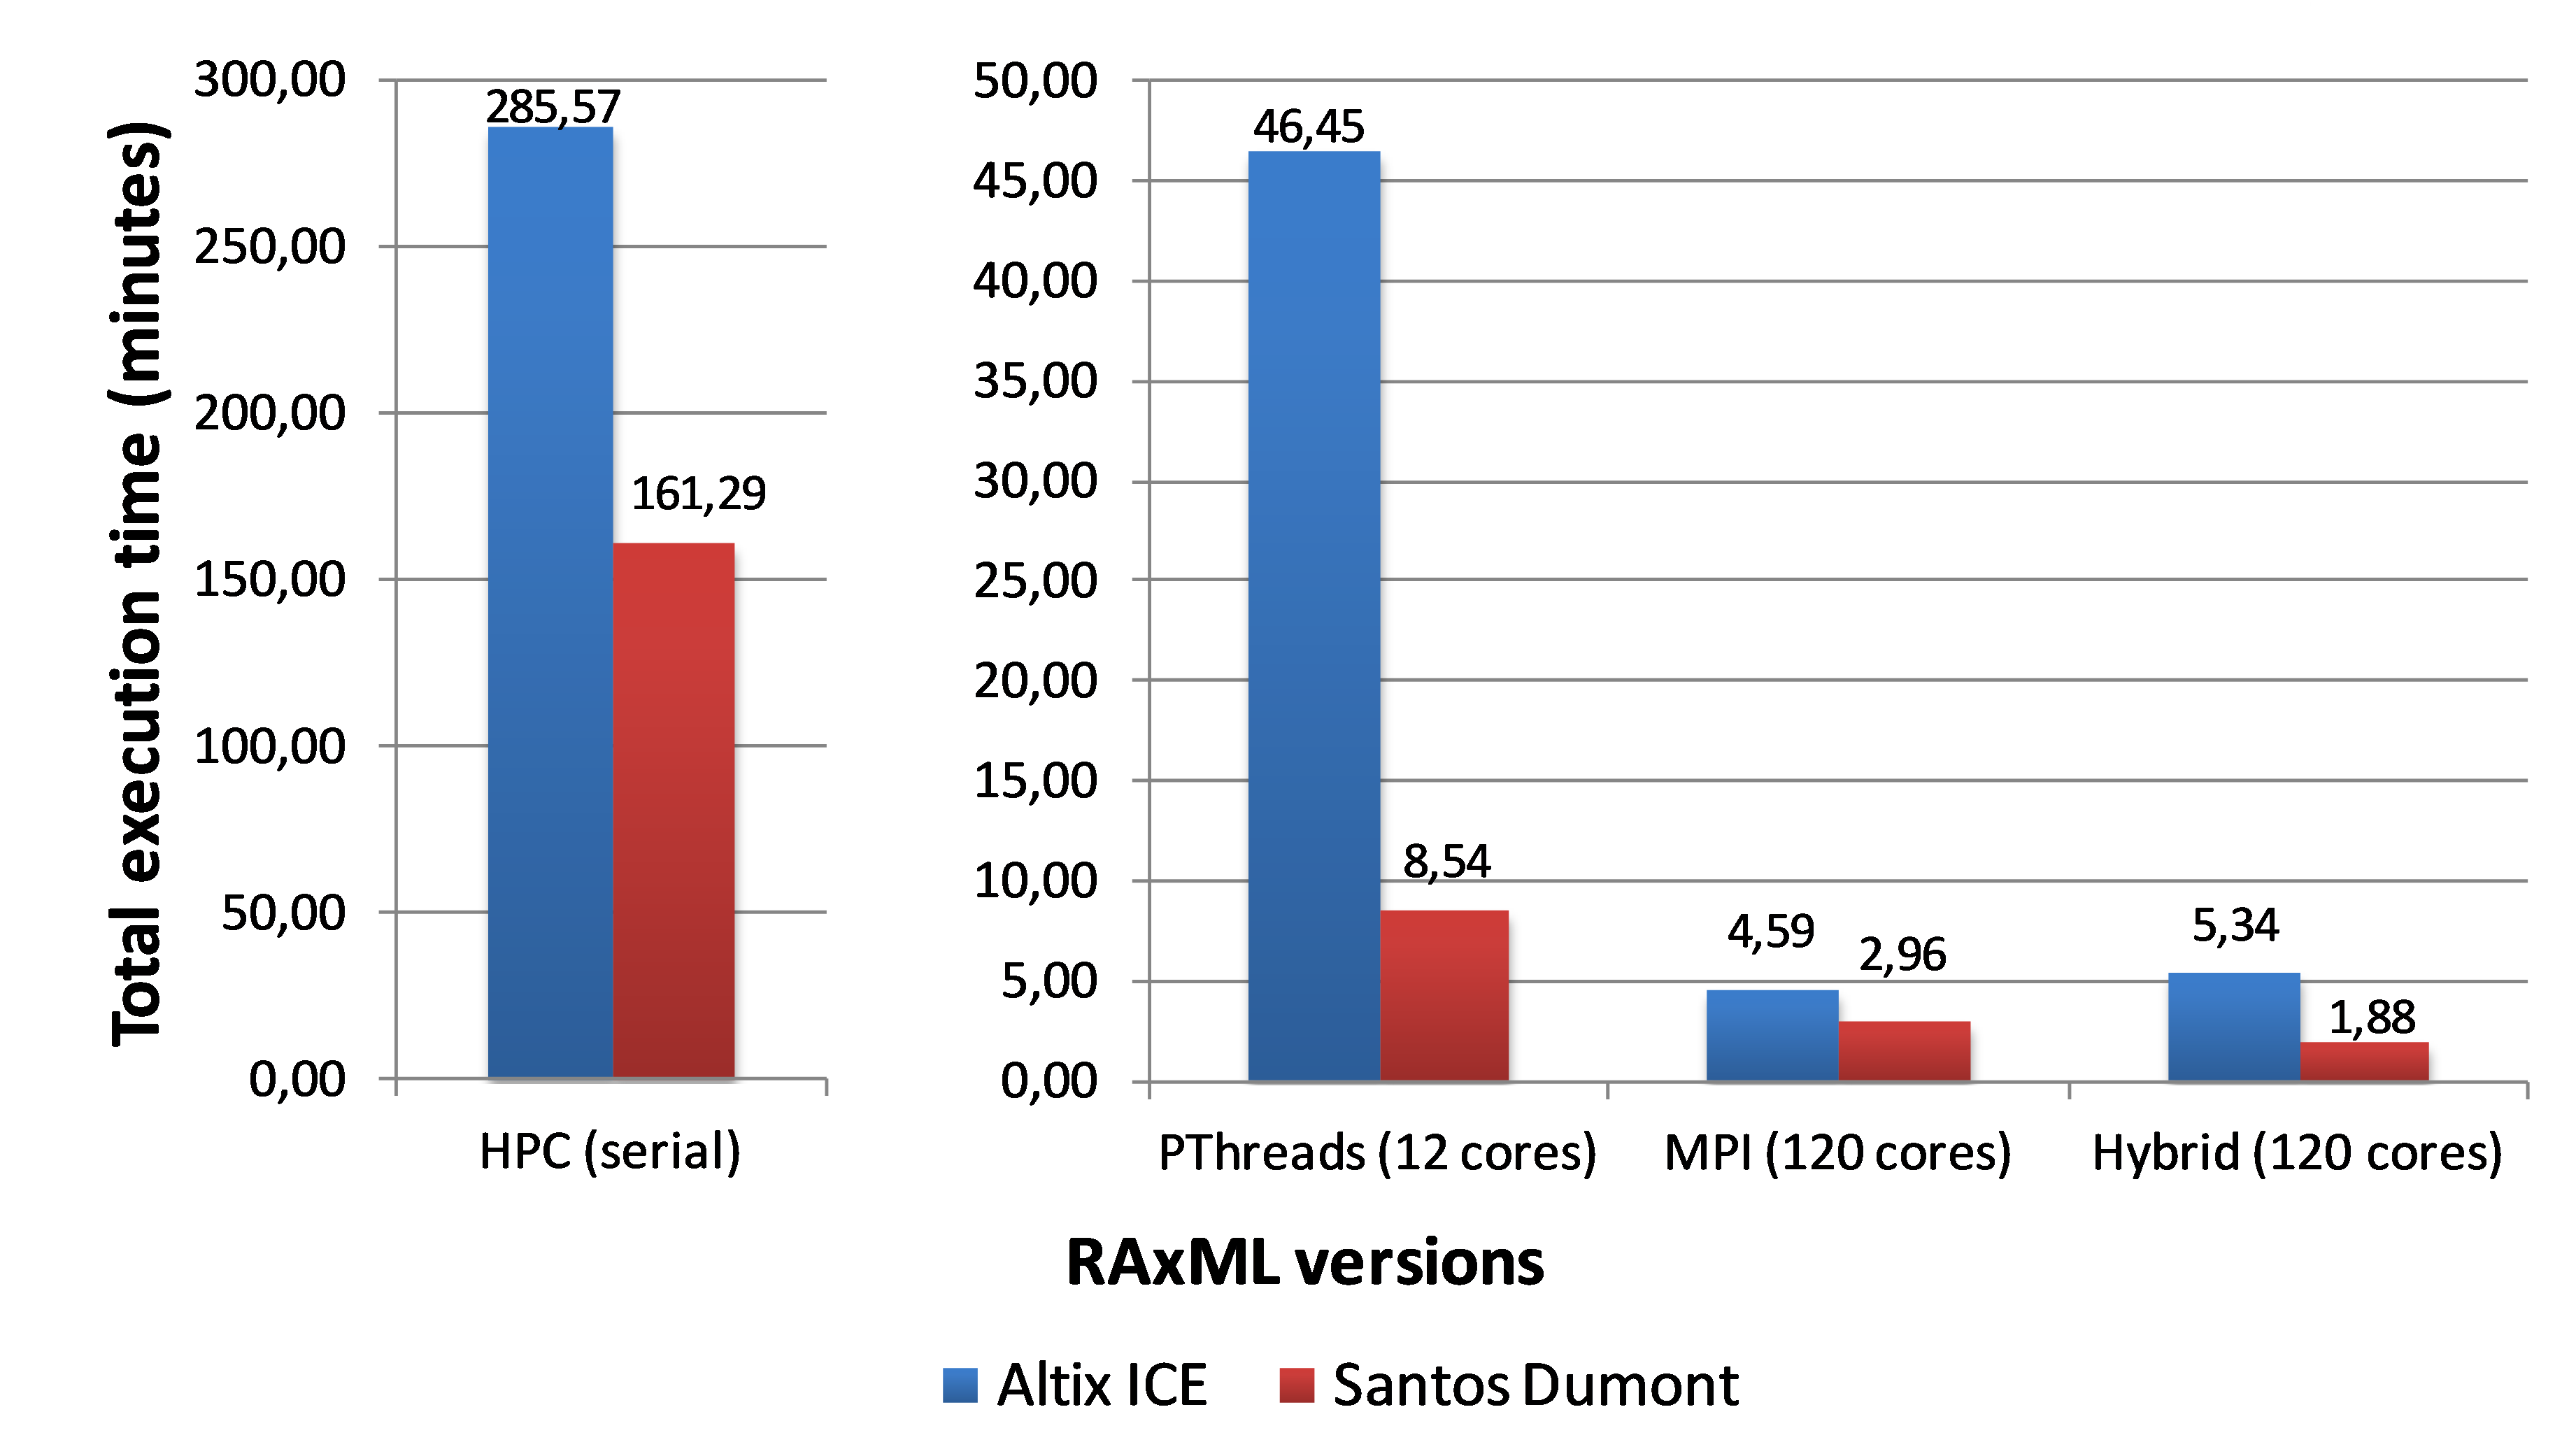
\includegraphics[width=0.6\textwidth]{imgs/raxmlTETD5.png}
\vspace{-12px}
\caption{\system performance (TET) results for \raxml in Altix and SDumont for the superalignment D5}
\label{fig:raxmlTETD5}
\end{figure}

\textit{2) The scalability of \raxml MPI (Altix) and \raxml Hybrid (SDumont)}. This experiment aims to evaluate the performance gains of the versions of \raxml that outperformed Altix (\raxml) and SDumont (\raxml Hybrid) according to the number of cores in minutes. The performance of \raxml was measured on a single processor machine (one core) to analyze the local optimization before scaling up the number of cores. After that, the performance and scalability of \raxml were measured using from 2 up to 120 cores. The superalignment used as input data is D5. Figure~\ref{fig:raxmlscalabilityD5} presents the scalability in minutes obtained after the execution of \raxml MPI in Altix and \raxml Hybrid in SDumont. The TET decreases, in both cases, as more cores were provided. \raxml Hybrid (SDumont) presented the best performance, the TET was reduced from 161.29 minutes (one single core) to 10.39 minutes (24 cores) and to 1.88 minutes (120 cores). Using one core, \raxml Hybrid at SDumont outperforms \raxml MPI at Altix; the TET was reduced from 285.57 minutes to 161.29 minutes.

\begin{figure}[!htb]
\centering
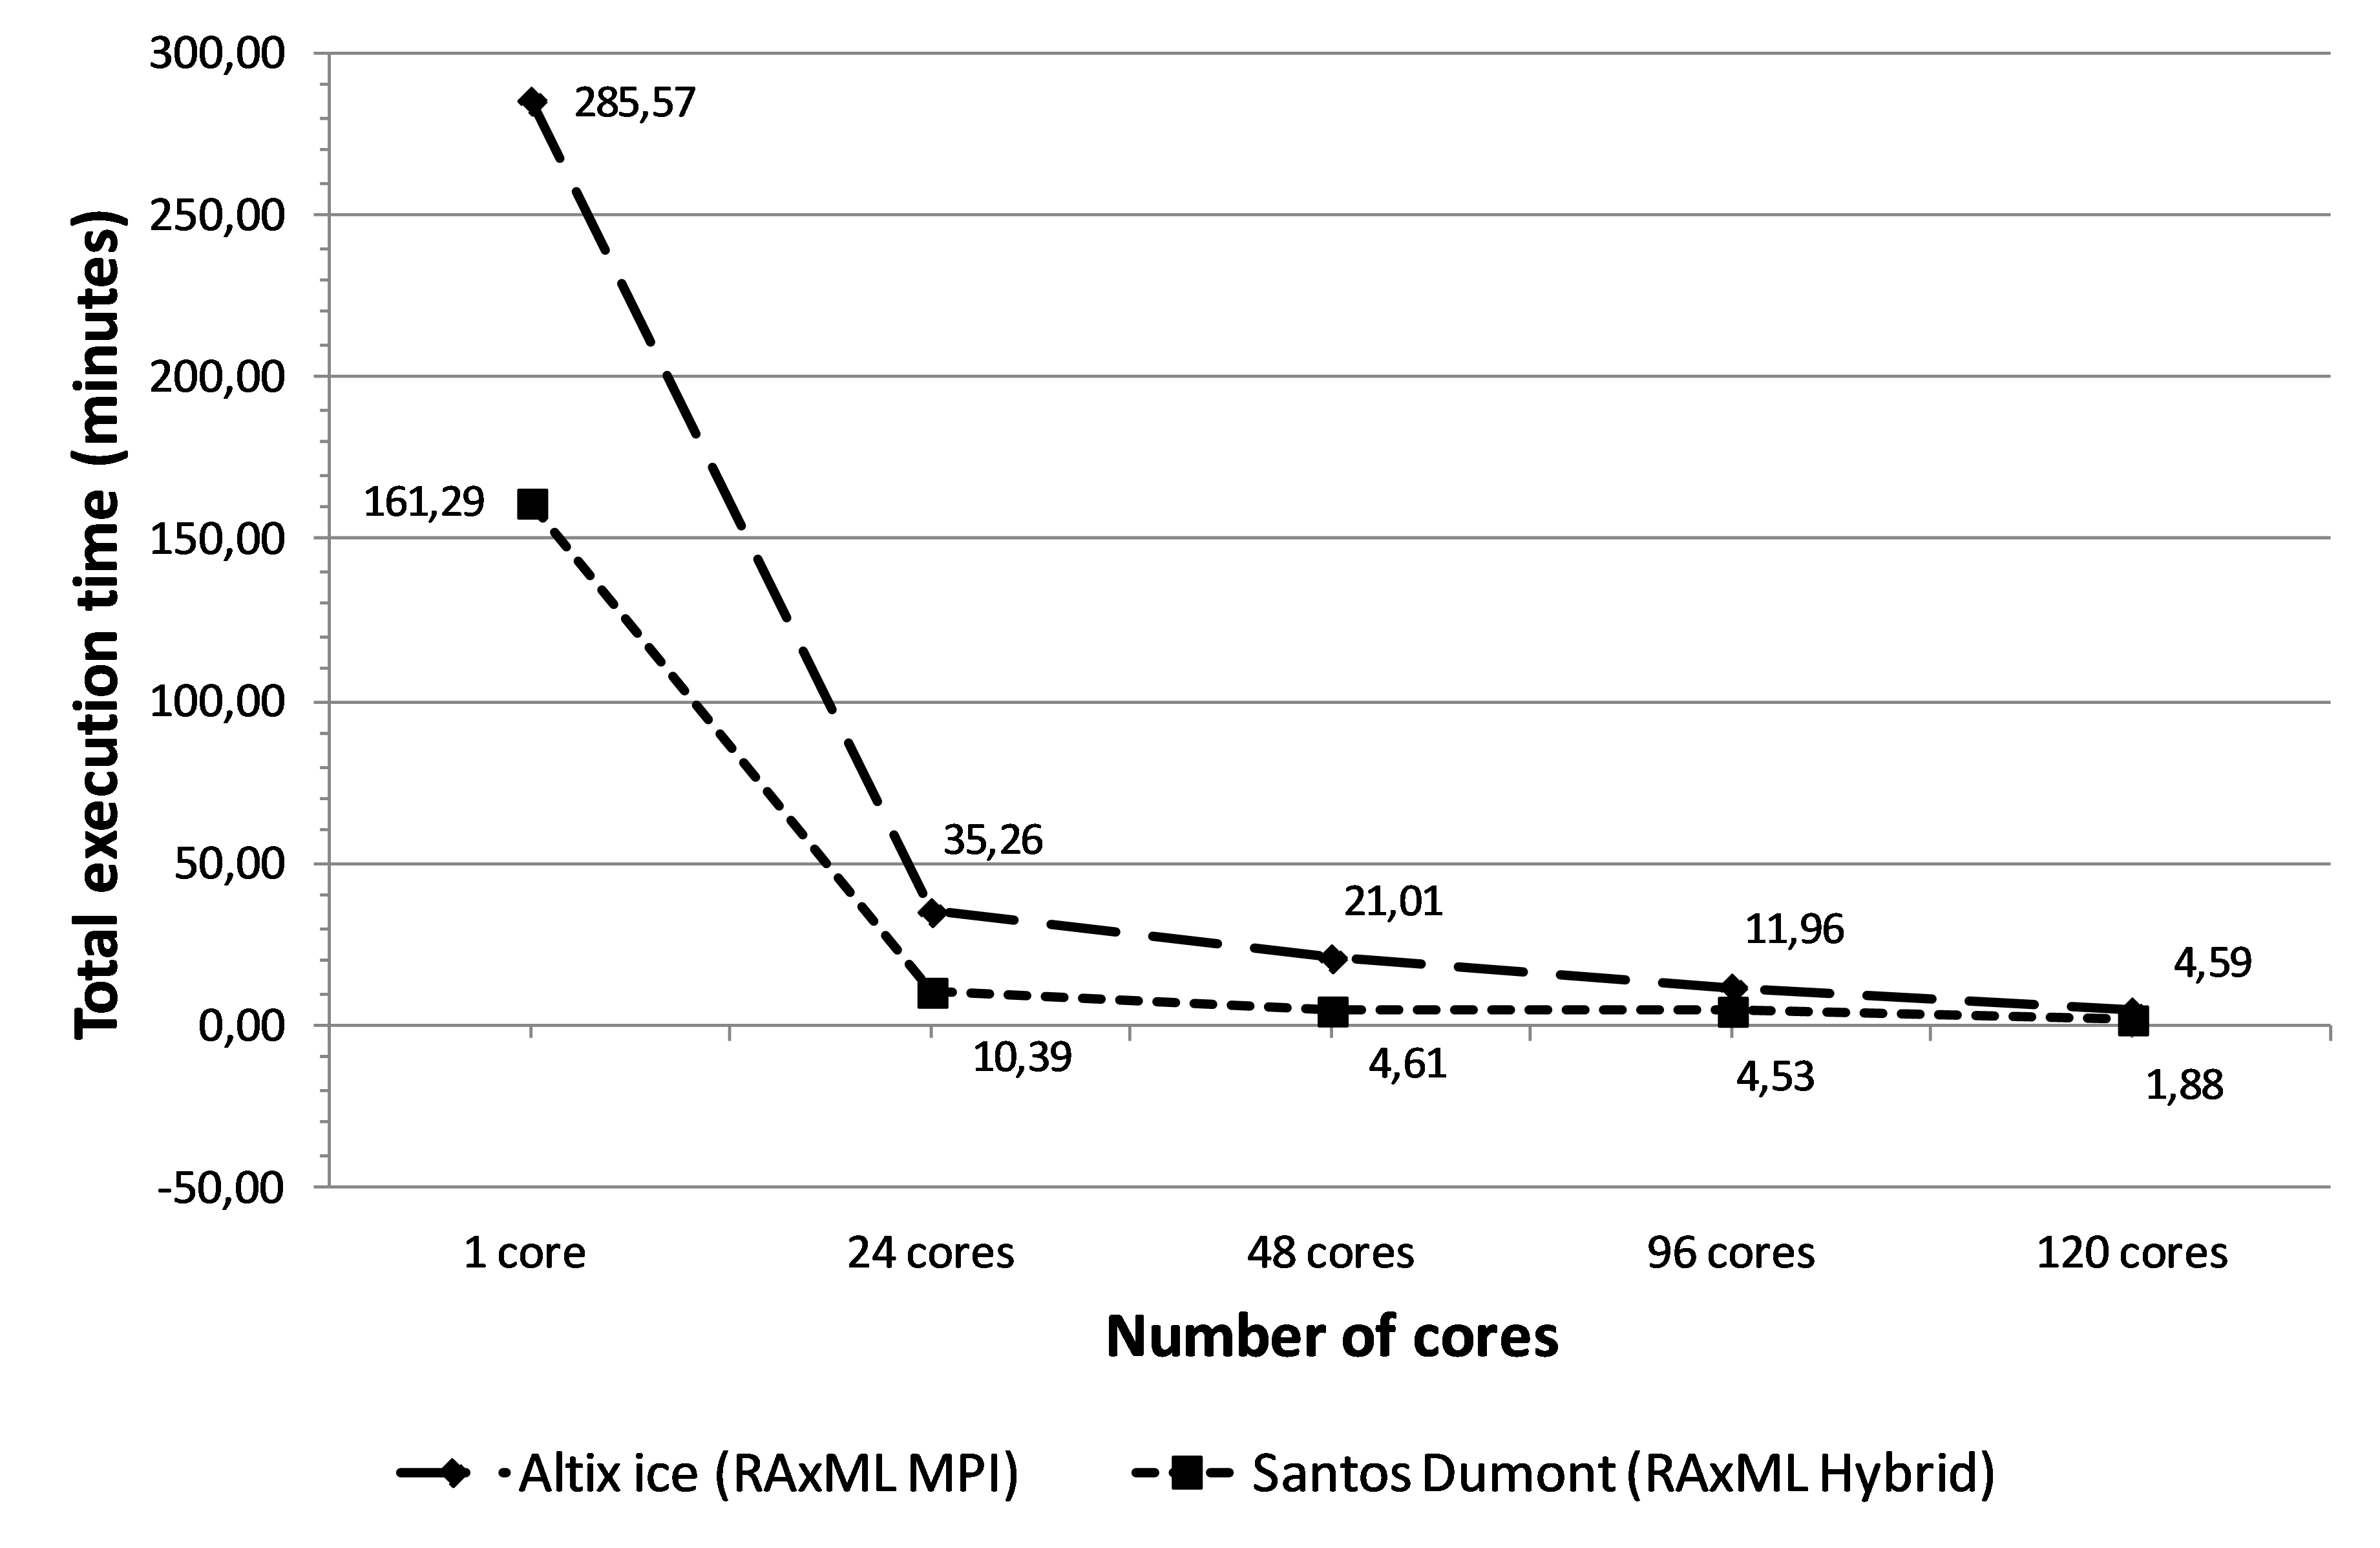
\includegraphics[width=0.6\textwidth]{imgs/raxmlscalabilityD5.png}
\vspace{-12px}
\caption{\system performance (scalability) results for \raxml MPI in Altix and \raxml Hybrid in SDumont for the superalignment D5}
\label{fig:raxmlscalabilityD5}
\end{figure}

\textit{3)The TET of \raxml MPI (Altix) and \raxml Hybrid (SDumont) using eight superalignments}. The executions of the \raxml versions used as input files eight superalignments, varying features of the number of taxa, number of amino acid, and size (KB). The parameters used for setting \raxml versions are JTT as the evolutionary model, GAMMA as the rate of the heterogeneity of the model, and 100 as the bootstrap value of replications. Figure~\ref{fig:raxmlTETAllD} presents the TET in hours of \raxml MPI and \raxml Hybrid in Altix using eight superalignments. The TET decreases, for all superalignments, when the \raxml parallel versions were executed. The eight superalignments files were categorized as Large (D1, D2), Medium (D3, D4, D7, D8), and Small (D5, D6). The versions \raxml MPI and \raxml Hybrid outperformed the versions \raxml HPC Serial and \raxml PThreads. With \raxml Hybrid, the TET of the largest file D1 was reduced from 820.60 hours (using one single core) to 30.10 hours (using 120 cores) and the TET of the smallest file D6 was reduced from 4.10 hours (using one single core) to 0.10 hours (using 120 cores). A relation was observed between the increment of the size of the superalignments files and the improvement of performance of approximately 90\% between 1 and 120 cores. D1: 2,091 KB and 96.33\%; D2: 1,260 KB and 95.99\%, D3: 792 KB and 95.78\%; D4: 553 KB and 95.47\%; D7: 168 KB and 95.63\%; D8: 157 KB and 94.75\%; D5: 95.83 KB and 97.83\%; D6: 72 KB and 97.50\%. These values indicate that parallelization benefits from larger files and that have more taxa and/or longer sequence lengths.

\begin{figure}[!htb]
\centering
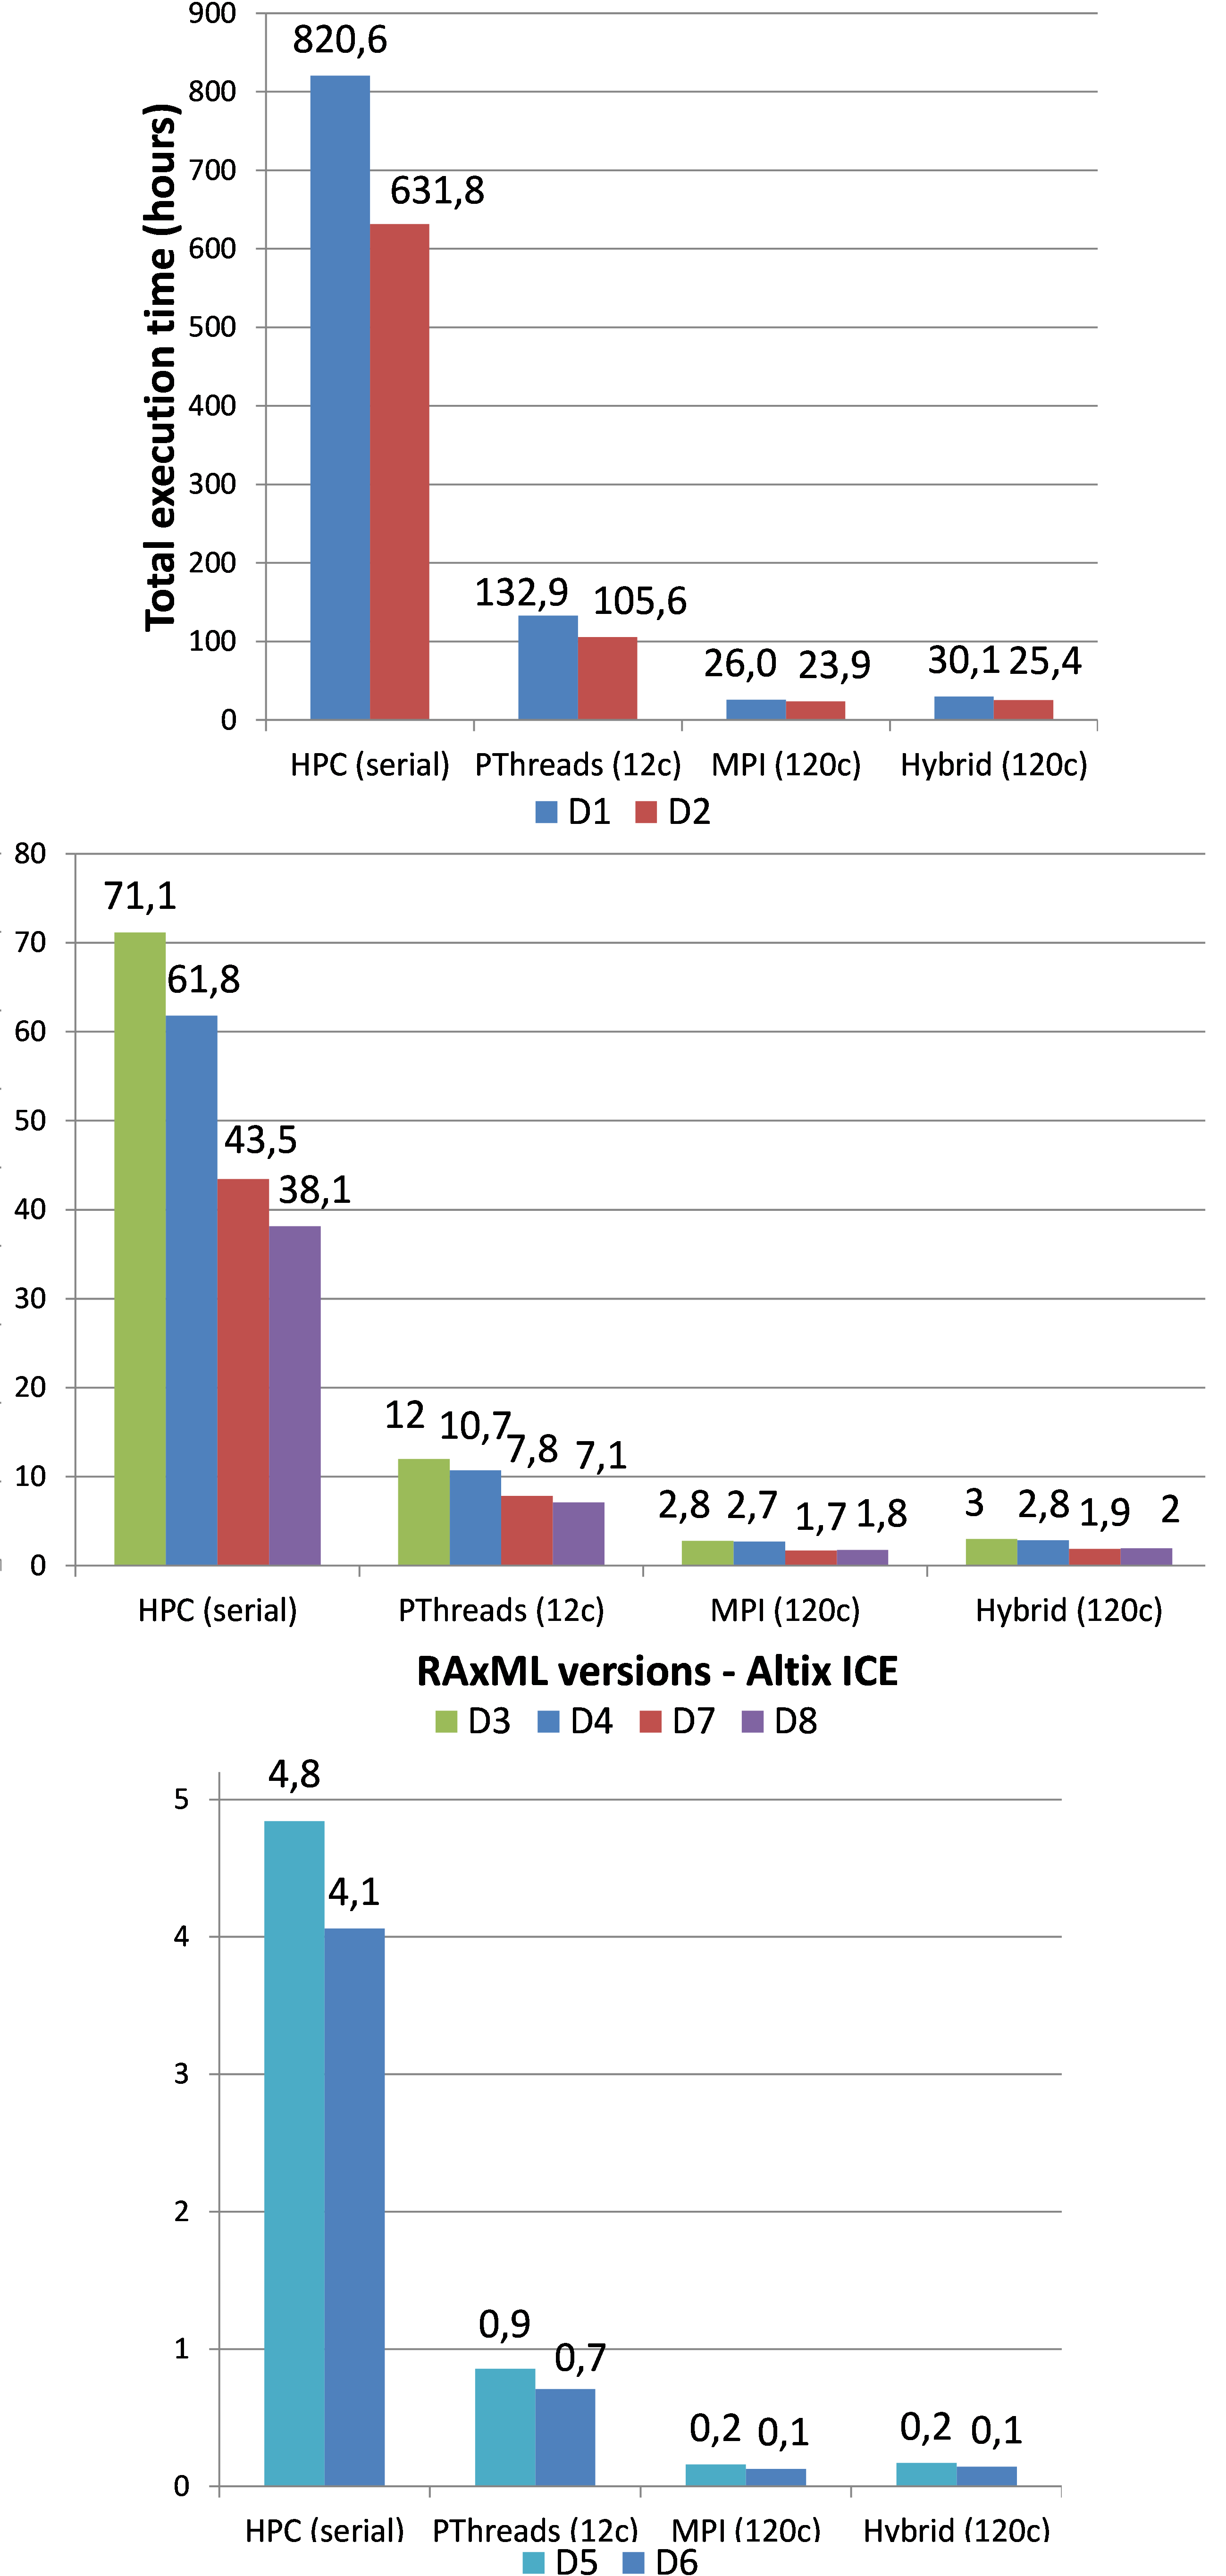
\includegraphics[width=0.6\textwidth]{imgs/raxmlTETAllD.png}
\vspace{-12px}
\caption{\system performance (TET) results for \raxml MPI and \raxml MPI in Altix for all eight superalignment}
\label{fig:raxmlTETAllD}
\end{figure}

\vspace{5px}
\noindent
\underline{\textbf{\sci}}, querying runtime the provenance database of SciCumulus allows to obtain the status of the \sci executions, which can be reported automatically as messages at the web interface \textit{e.g.} which activity is finished or if an error is presented. The arguments used as input files and parameters required to execute \sci through \system are: to upload the input file (alignment in FASTA format) and to fill the following options, input file type (\textit{e.g.} amino acid), e-mail, and output directory. Figure~\ref{fig:raxmlTETAllD} shows print messages at the final of each activity execution of \sci at \system, obtained by querying the SciCumulus provenance database. The activities that were successfully finished were printed in the web interface in green; on the other hand, those ones that reported an error in the execution were printed in red. 

\begin{figure}[!htb]
\centering
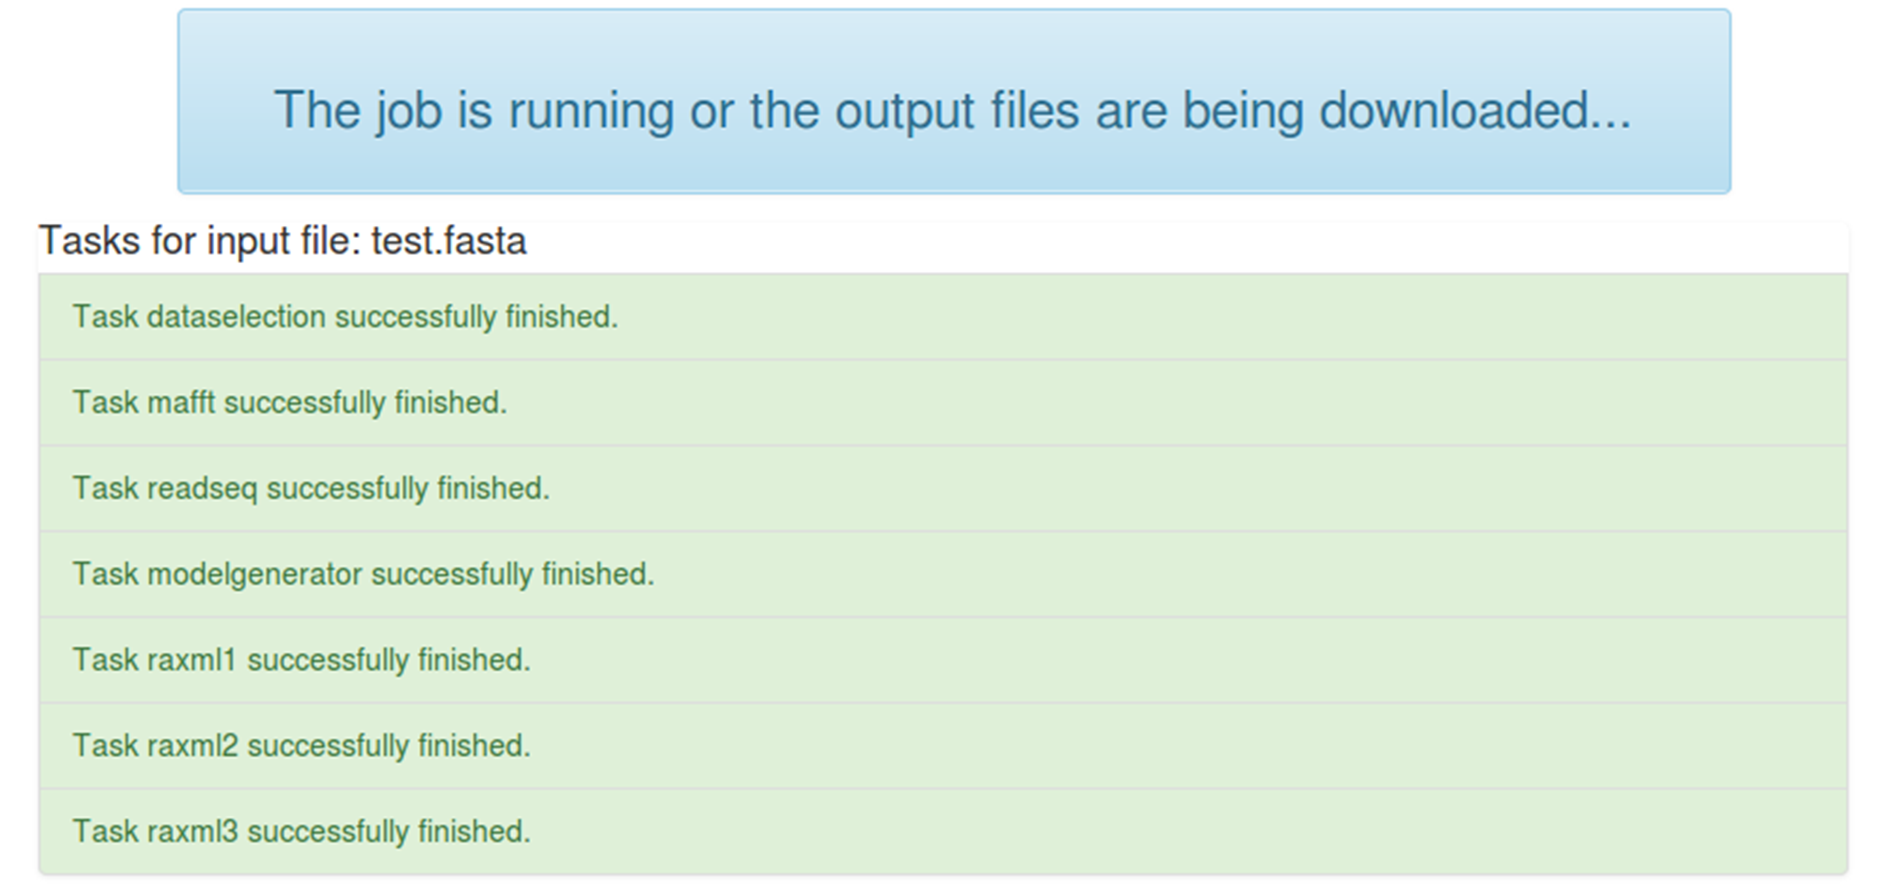
\includegraphics[width=0.6\textwidth]{imgs/sciphyoutputbioinfo.png}
\vspace{-12px}
\caption{\system output for \sci executions}
\label{fig:sciphyoutputbioinfo}
\end{figure}

We have evaluated the performance of the parallel execution of \sci in Altix. \sci was executed with 200 multifasta input files of amino acid sequences and three different configurations: on a single processor cluster (16 cores) through \system, on a single processor cluster (16 cores) directly at the cluster through CSGrid, and on three processor clusters (16 cores each) directly at the cluster through CSGrid. Figure~\ref{fig:sciphyTET} presents the TET in minutes of \sci, which presents the best performance with the third configuration \textit{i.e.} when it is executed directly at CSGrid with three clusters (in green). The TET was reduced from 374.75 minutes (using one single cluster through \system) to 180.19 minutes (using three clusters through CSGrid).

\begin{figure}[!htb]
\centering
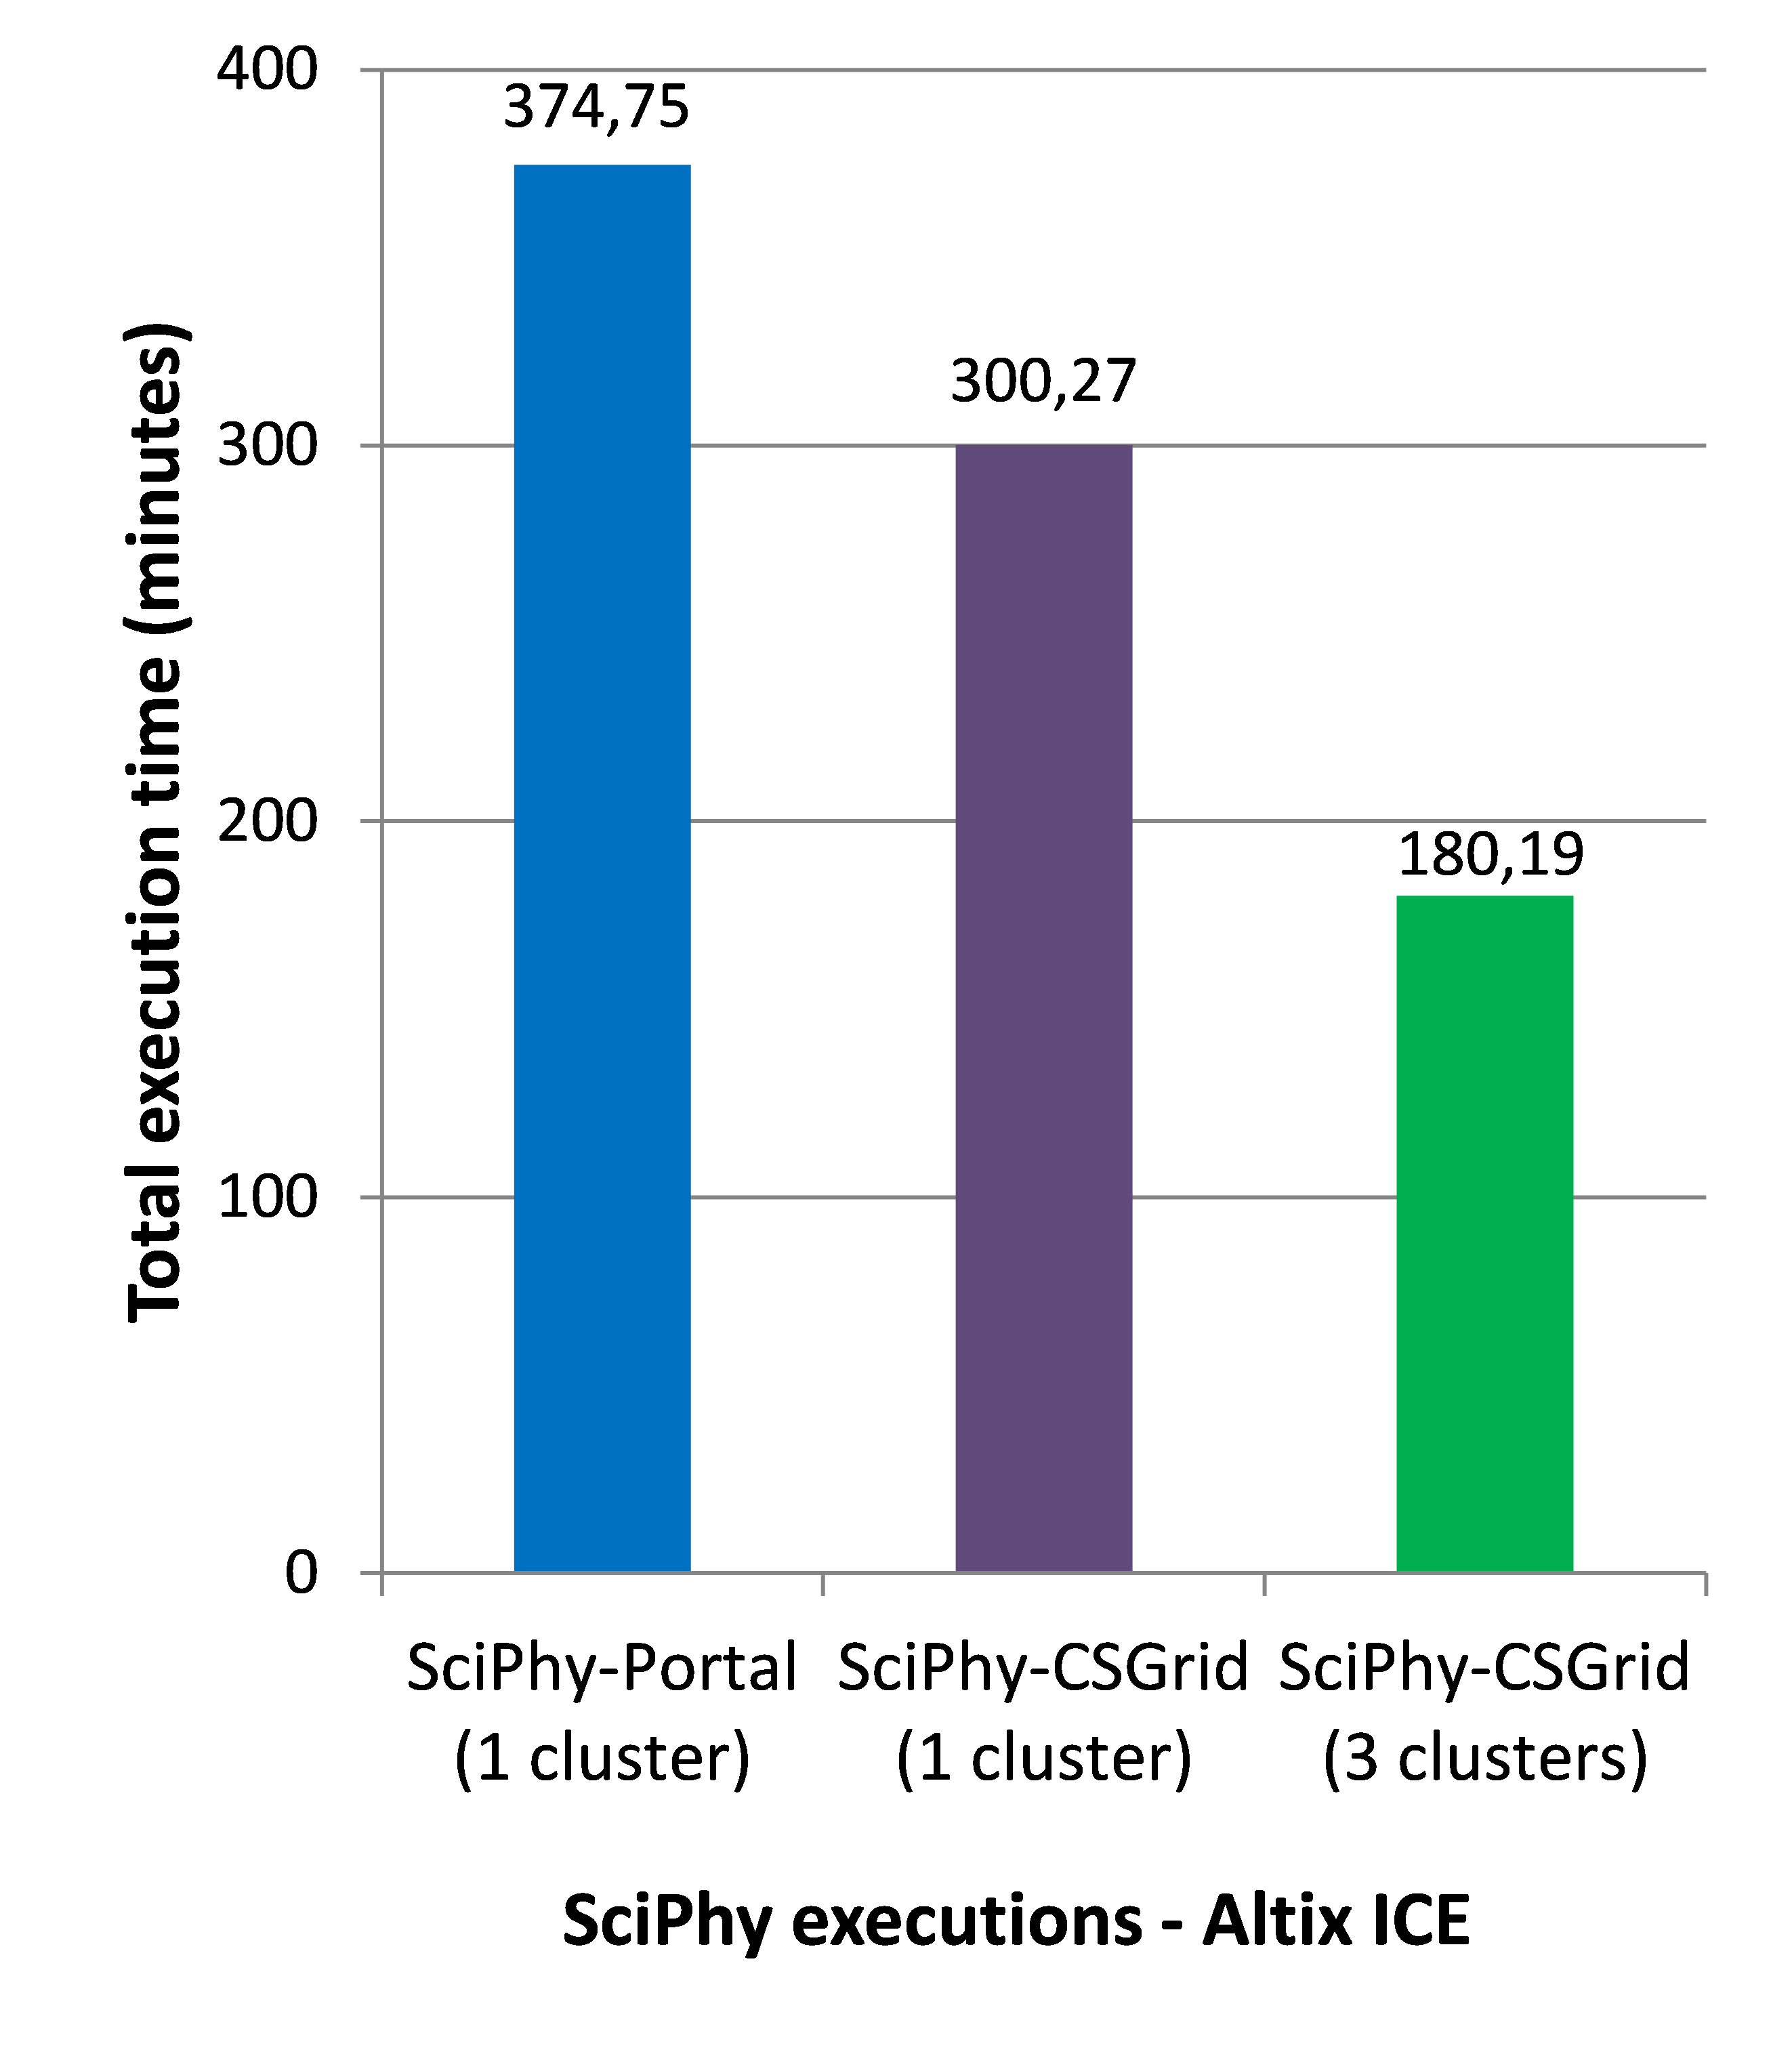
\includegraphics[width=0.6\textwidth]{imgs/sciphyTET.png}
\vspace{-12px}
\caption{\system output for \sci executions}
\label{fig:sciphyTET}
\end{figure}


\vspace{5px}
\noindent
\underline{\textbf{\swift}}, executions (resulting in 135 task executions) were performed in a cluster with 72 nodes, 16GB of RAM, and eight computing cores per node. The input data is formed by five genomes of bacteria completely annotated. The TET was based on three metrics: a sequential execution directly at the cluster (in red); a parallel execution directly at the cluster (in blue); and a parallel execution through CSGrid via \system (in green). Figure~\ref{fig:swiftgeckoTET} presents the TET in minutes of \swift, which presents the best performance with the second configuration \textit{i.e.} using a parallel execution directly at the cluster (in blue). The TET was reduced from 8.2 minutes (sequential execution directly at the cluster) to 4.23 minutes (parallel execution directly at the cluster). Experiments in Figure~\ref{fig:swiftgeckoTET} also shows that invoking a CSGrid function via \system introduces a small run-time overhead compared to parallel execution time. It is worth mentioning that \swift applications use an out-of-core strategy and are I/O intensive. Then, scalability could be improved by using higher throughput storage systems or more efficient data management strategies. Finally, the parallel execution through CSGrid via \system measures the time required for submission, execution, and file transference between CSGrid/SINAPAD and the cluster, which increment the time of response via \system.

\begin{figure}[!htb]
\centering
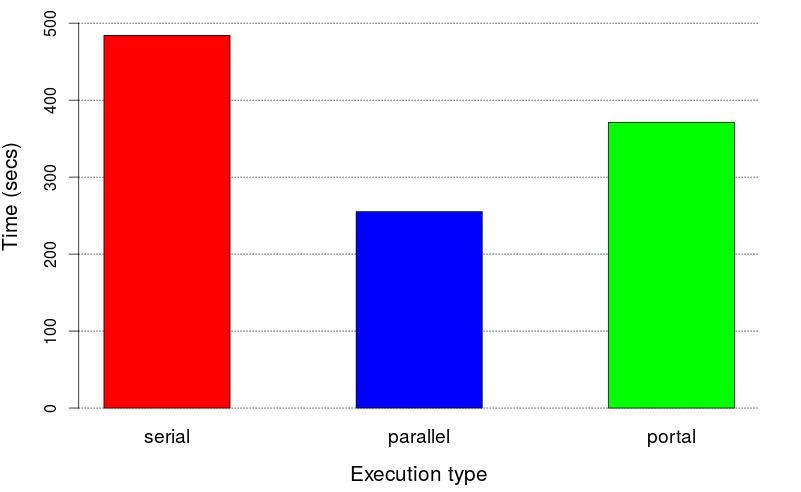
\includegraphics[width=0.6\textwidth]{imgs/swiftgeckoTET.png}
\vspace{-12px}
\caption{\system output for \swift executions}
\label{fig:swiftgeckoTET}
\end{figure}

\subsection{\system data analysis using machine learning}

The database of Bioinfo and provenance databases of the SWfMS were integrated into the statistical tools of Google Analytics. The information of jobs executed per month, jobs executed per applications, or session per country can be accessed to \system. Figure~\ref{fig:bioinfoTET} shows the TET in hours per applications executed until 01/11/2018. The applications most accessed were FragGeneScan, Align-m, and Phylip. Until 01/02/2019, the portal was accessed 2,812 times and 766 applications were executed.

\begin{figure}[!htb]
\centering
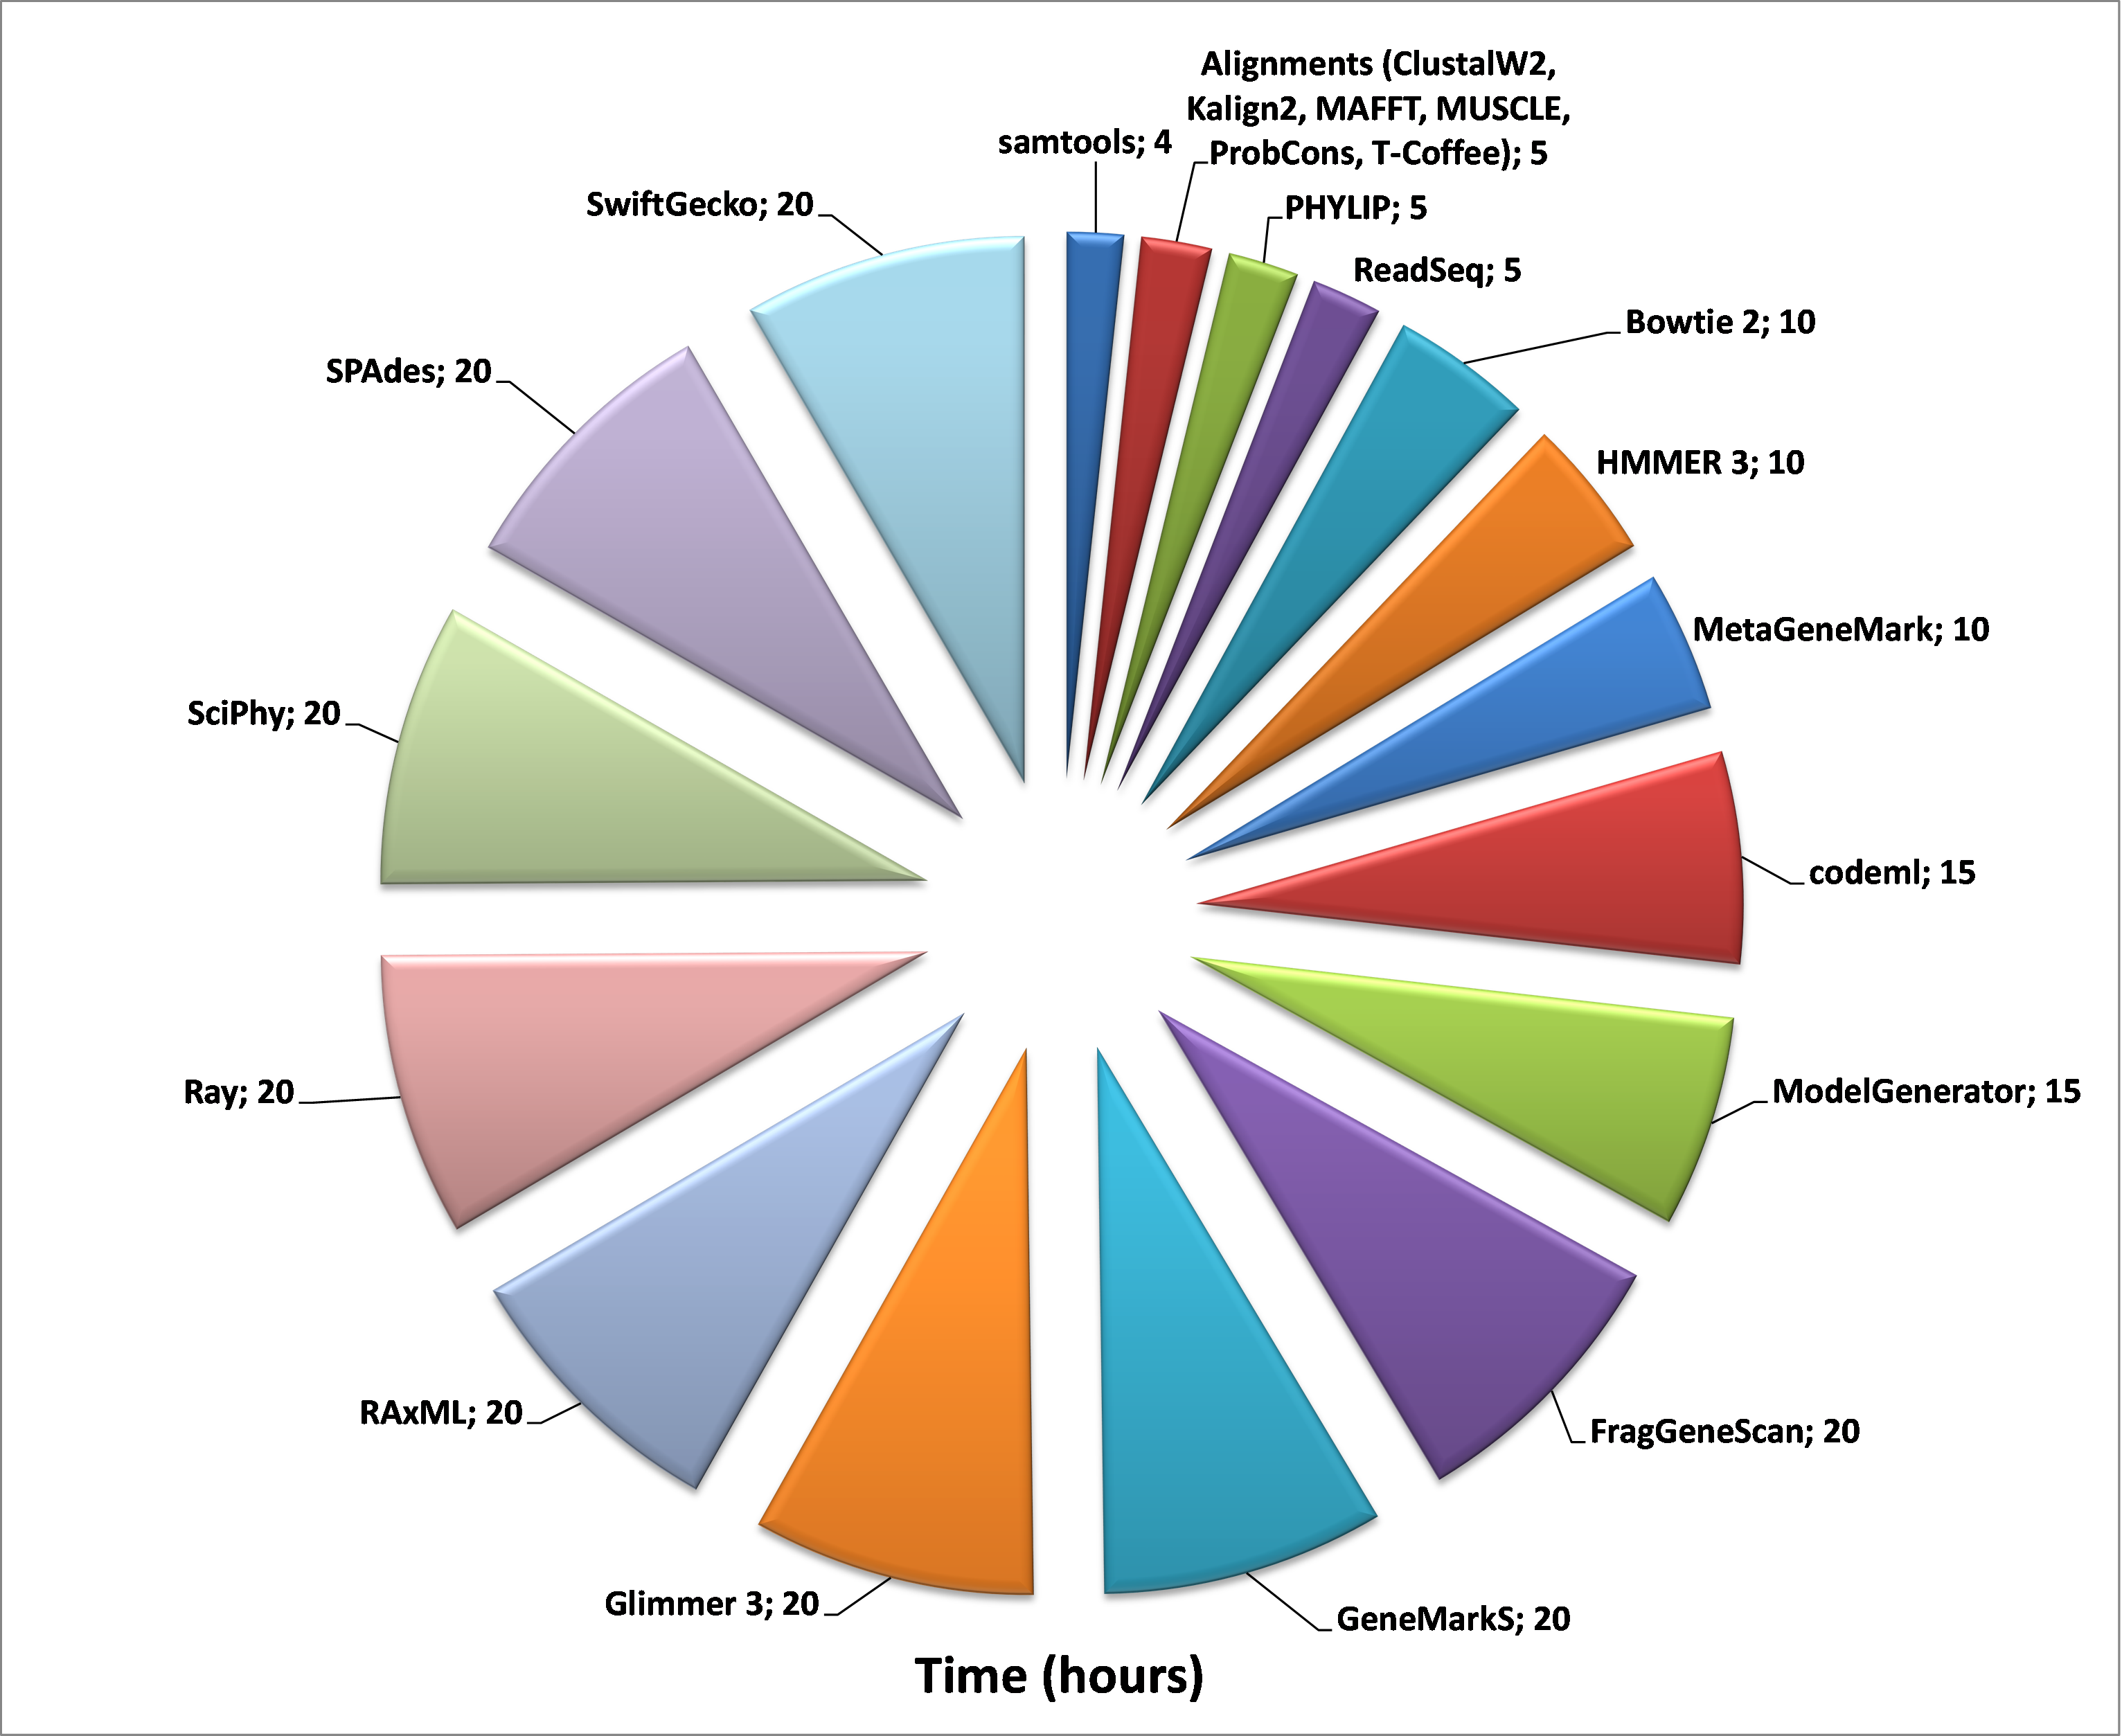
\includegraphics[width=0.6\textwidth]{imgs/bioinfoTET.png}
\vspace{-12px}
\caption{\system output for \swift executions}
\label{fig:bioinfoTET}
\end{figure}

An exploratory data analysis using classification trees was performed with the available data of the database of \system to infer knowledge about the most adequate computational resource to execute the applications. Data mining algorithms were used to discover patterns; we apply regression models with decision trees [22] using the Orange data mining tool for statistical analyses. Orange implements the core algorithm ID3 and employs a top-down, greedy search through the space of possible branches with no backtracking. Nevertheless, before generating the decision tree, we had to evaluate the statistics that each attribute used in the model (\textit{i.e.} threads, datasize, node attributes). The main idea of the attribute analysis is to identify potential problems with the chosen attributes and decide if an action needs to be taken that may require collecting more data. In Figure~\ref{fig:bioinfoTET}(a),(b),(c), we can state that there is no one dominant attribute value and the distribution is not even; and for our analyses, results indicate that attributes can be used in the predictions.

Figure~\ref{fig:bioinfoTET}(a) evaluates the threads attribute. We can observe that 75\% of the number of threads used was 24, from an interval of 24 to 240. Figure~\ref{fig:bioinfoTET}(b) shows that 75\% of data input presented size of 204 KB, from an interval of 3.2 to 610,000. Moreover, evaluating the node attribute in Figure~\ref{fig:bioinfoTET}(c), we observed that 75\% of the number of nodes used was 1, from an interval of 1 to 10. This information can assist users to distinguish outlier points to find anomalies or specific biological characteristics. By using these attributes to build estimation models, we can discover, using classification or regression algorithms, the relation of biological input data (size in KB) and the number of threads that can be used for the executions that generate maximum values of efficiency. Now we observed that the applications of \system consume low computational resources, which is due to the restriction for size and number of inputs assigned to the Projects of users.

\begin{figure}[!htb]
\centering
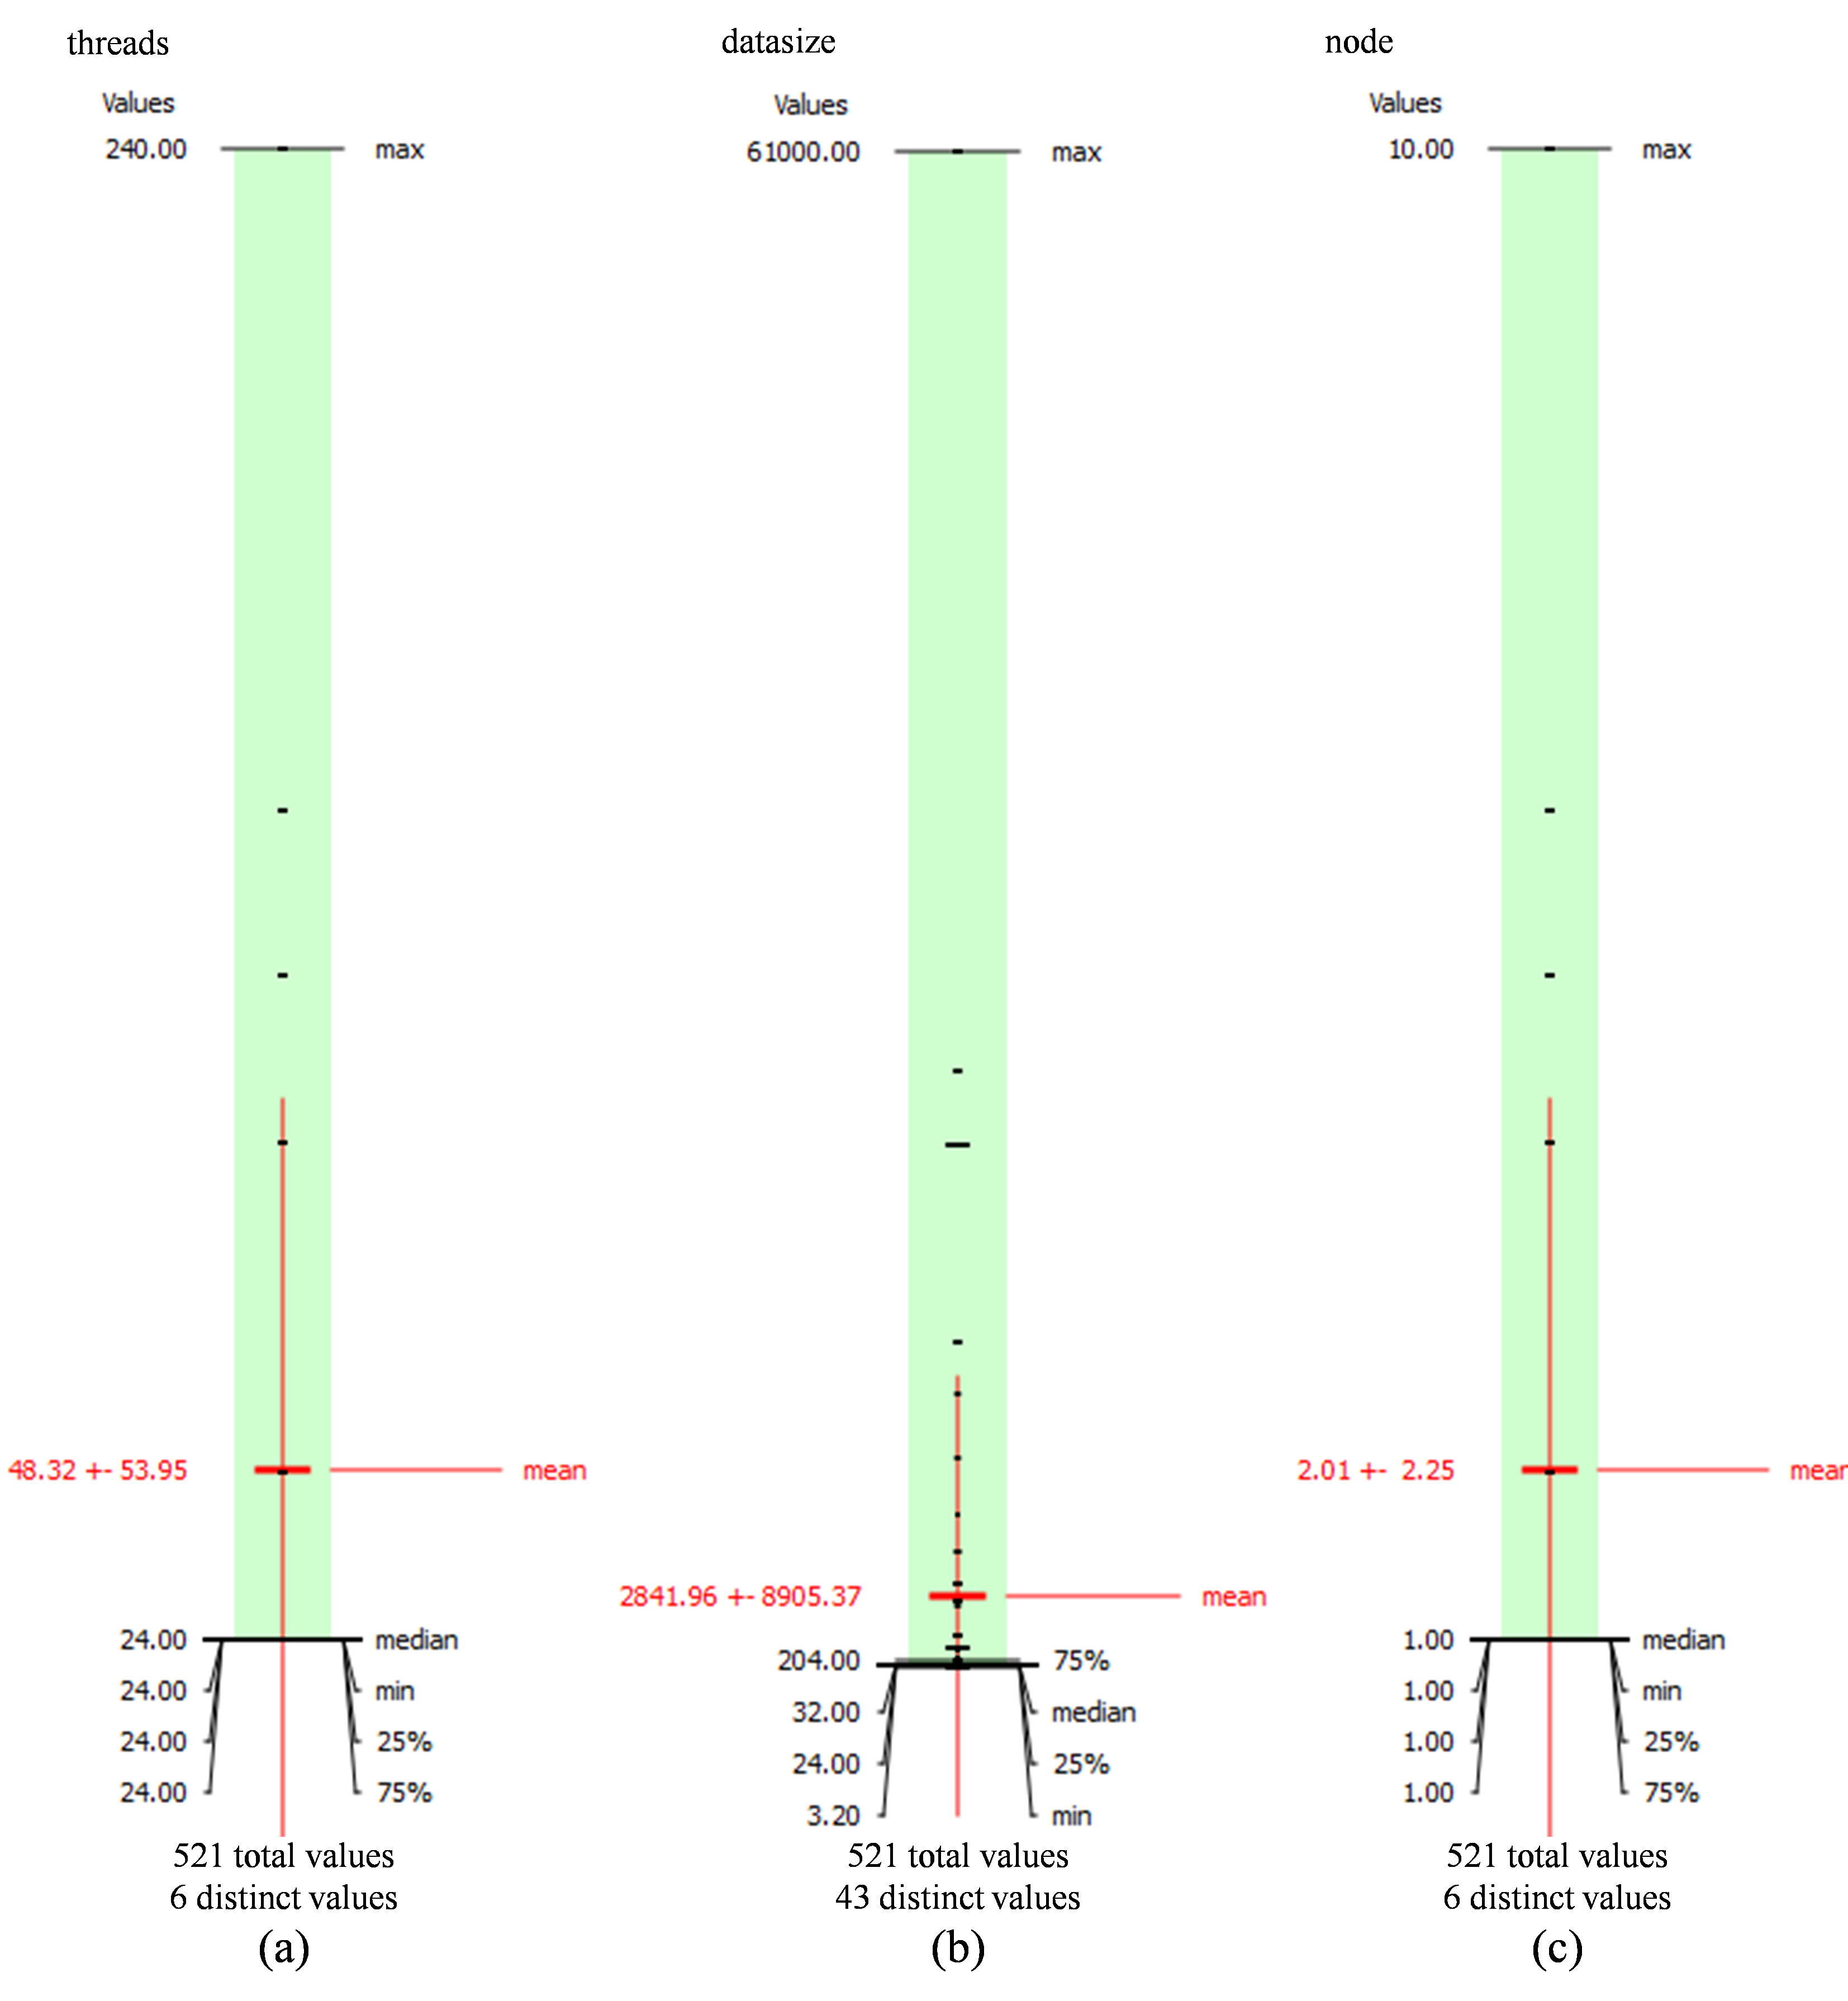
\includegraphics[width=0.7\textwidth]{imgs/mlattributes.png}
\vspace{-12px}
\caption{\system attribute statistics: (a) threads (number of threads), (b) datasize (data size of the alignment in KB), and (c) node (number of nodes)}
\label{fig:mlattributes}
\end{figure}

Figure~\ref{fig:mldecisiontree} presents the inferred rules for exploring the efficiency of the executions of applications at \system. In this analysis, we can state that the efficiency of computational resources of \system applications is determined by two parameters: the number of threads (threads), the size of the alignment in KB (datasize), and the number of nodes (node) \textit{i.e.} the combination of values of these three parameters defines the efficiency of the executions. 
For example, Figure~\ref{fig:mldecisiontree} presents that the efficiency that consumes the number of threads between 100 and 81 with less than 36,000 of size in KB of data size and will obtain, on average, 100 of efficiency. The machine-learning strategies appoint, for the actual scenario, that the best machine setup in a heterogeneous environment for executing applications presented at least 75\% of efficiency. However, results obtained are interesting and provide an idea about the behavior of application executions in HPC computational resources via \system, more refined experiments with more data must be reevaluated in future analyses. 

\begin{figure}[!htb]
\centering
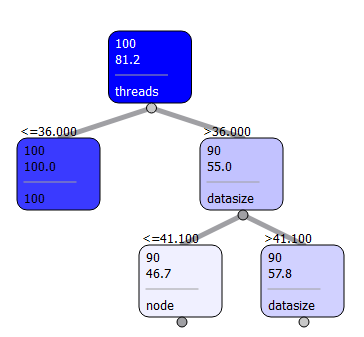
\includegraphics[width=0.6\textwidth]{imgs/mldecisiontree.png}
\vspace{-12px}
\caption{\system attribute statistics: (a) threads (number of threads), (b) datasize (data size of the alignment in KB), and (c) node (number of nodes)}
\label{fig:mldecisiontree}
\end{figure}


\section{Conclusions and Future Work}\label{sec:conclusions}


Although Apache Spark is a widely adopted DISC system for big data analytics and in-memory processing, it still lacks support for provenance management. 
This manuscript introduced \system, a solution that aims at fulfilling that gap and provide the support for running scientific workflows with provenance.
\system was carefully designed to handle prospective, retrospective, and domain data at runtime without jeopardizing Apache Spark overall performance.
Accordingly, we discussed and implemented an in-memory file system, called \texttt{SAMbA-FS}, which not only optimizes the execution of workflows with black-box applications as activities but also enables Apache Spark to become aware of contents produced by those external programs.
Experts can seamless instantiate \texttt{RDD Schemas} for the extraction of data elements produced by transformations that are further stored according to a \texttt{PROV-Df}-compliant model.
Persisted provenance data are retrieved at runtime by \textit{web} reports and can be queried by high-level SQL statements after the end of the experiments.
We evaluated \system on three real-world scientific workflows (\word, \montage, and \sci) and results indicated: 
\textit{(i)}~\system did not jeopardize standard Apache Spark performance, and 
\system{(ii)}~\system efficiently provided runtime and \textit{post-mortem} data analytics.
%Accordingly, we believe \system can turn Apache Spark into an even more attractive alternative for the running of scientific workflows. 
Future work includes adapting the \system design to collect provenance from Data Frames as many applications are moving towards to them.


% Apache Spark is a widely adopted DISC system for big data analytics and its in-memory processing, large installation base, and support has attracted IO intensive scientific workflows to benefit from data parallelism, scheduling strategies and fault tolerance mechanisms.
% However, Apache Spark is still limited in supporting data provenance and analysis. \system contributes to current approaches in providing provenance to Spark by capturing prospective, retrospective, and domain data provenance during the workflow execution.
% In addition, SAMBA also extracts raw data selected from files by an efficient file system named \texttt{SAMbA-FS}.

% We modeled the gathered provenance data by using the \texttt{PROV-Df} model.
% Moreover, \system supports provenance management by properly handling both the structure and content of Spark RDDs.
% Experts can instantiate \texttt{RDD Schemas} for the extraction of data elements produced by black-boxes transformations.
% \system uses an in-memory file system that improves I/O operations demanded by black-box programs of scientific workflows and efficiently provides users with runtime querying and \textit{post-mortem} data analytics.
% %\system relies on an in-memory file system that improves I/O operations demanded by black-box programs of scientific workflows so that our approach efficiently provides runtime querying and \textit{post-mortem} data analytics.

% We evaluate \system in a practical scientific workflow on bioinformatics domain called \texttt{SciPhy} and results indicated: (i) \system did not jeopardize standard Apache Spark performance, and (ii) \system efficiently provided runtime and \textit{post-mortem} data analytics.

% We believe that \system can make the use of Apache Spark even more attractive for the classes of IO-intensive scientific workflows. 
% Future work includes the evaluation of \system with different scientific workflows, such as Montage~\cite{montage}. We also plan to investigate how to collect provenance from Data Frames as many applications are moving toward to them.

% \section*{Acknowledgments}






%% The Appendices part is started with the command \appendix;
%% appendix sections are then done as normal sections
%% \appendix

%% \section{}
%% \label{}

%% References
%%
%% Following citation commands can be used in the body text:
%% Usage of \cite is as follows:
%%   \cite{key}         ==>>  [#]
%%   \cite[chap. 2]{key} ==>> [#, chap. 2]
%%

%% References with BibTeX database:

\bibliographystyle{elsarticle-num}
\bibliography{ref}

%% Authors are advised to use a BibTeX database file for their reference list.

%% For references without a BibTeX database:

% \begin{thebibliography}{00}

%% \bibitem must have the following form:
%%   \bibitem{key}...
%%

% \bibitem{}

% \end{thebibliography}

\end{document}

%%
%% End of file `ecrc-template.tex'. 